% ============================================================
% PRESENTACIÓN VISUAL (Claude) — para proyectar
% Poco texto en pantalla, imágenes grandes y transiciones entre
% diapositivas. El texto de apoyo para exponer está en las notas
% de beamer (visibles solo en presentacion_claude_texto.tex).
% ============================================================
\documentclass[aspectratio=169]{beamer}
\usepackage[spanish]{babel}
\usepackage[utf8]{inputenc}
\usepackage{tikz}
\usetikzlibrary{shapes.geometric}
\usepackage{circuitikz}
\usepackage{booktabs}
\usepackage{amsmath}
\usepackage{amssymb}
\usepackage{svg}
\usepackage{graphicx}
\graphicspath{{imagenes/}}

\usetheme{Berkeley}
\usecolortheme{default}

\title[LCL Conmutado]{Diseño, modelado e implementación de un circuito conmutado para la protección por sobre-corriente}
\subtitle{Trabajo de Fin de Grado}
\author[Á. Villalta]{Álvaro Villalta Vázquez}

\institute[UC3M]{
  Grado en Ingeniería Electrónica Industrial y Automática\\
  Universidad Carlos III de Madrid\\[4pt]
  \textit{Tutora:} Cristina Fernández Herrero
}

\date[2025-2026]{Leganés, 2026}
\logo{
\includegraphics[width=1.4cm]{logo-universidad.png}}

\AtBeginSection[]
{
  \begin{frame}
    \transwipe
    \frametitle{Índice}
    \tableofcontents[currentsection]
  \end{frame}
}

\begin{document}

%--------------------------------------------------------------
% 1. PORTADA
%--------------------------------------------------------------
\frame{\titlepage}

%--------------------------------------------------------------
% 2. ÍNDICE GENERAL
%--------------------------------------------------------------
\begin{frame}
\transwipe
\frametitle{Índice}
\tableofcontents
\end{frame}

%--------------------------------------------------------------
% 3. CONTENIDO (compartido con la versión con notas)
%--------------------------------------------------------------
% ============================================================
% CONTENIDO COMPARTIDO DE LA PRESENTACIÓN (Claude)
% Este fichero es incluido (\input) tanto por presentacion_claude.tex
% (versión visual, para proyectar) como por presentacion_claude_texto.tex
% (versión reducida con el texto de apoyo debajo de cada diapositiva).
% No compilar directamente: no contiene preámbulo ni \begin{document}.
%
% Convención de revelado progresivo: cada elemento nuevo (viñeta,
% imagen, fórmula...) aparece tras un \pause, generando una
% transición cada vez que se añade contenido nuevo a la diapositiva.
% ============================================================

%==============================================================
\section{Introducción}
%==============================================================

\begin{frame}
\transdissolve
\frametitle{¿Qué es un LCL?}

\begin{columns}[c]
\column{0.54\textwidth}
\begin{block}{Latching Current Limiter (LCL)}
\small Protección de estado sólido ante sobrecorrientes entre bus de potencia $\longleftrightarrow$ carga.
\begin{itemize}\small
  \item<2-> \textbf{Limitación:} para $I~>~I_\text{lim}$.
  \item<3-> \textbf{Temporización:} limitación durante \textit{trip-off time}.
  \item<4-> \textbf{Enclavamiento:} ante fallo permanente.
\end{itemize}
\end{block}
\column{0.46\textwidth}
\onslide<5->{%
\centering
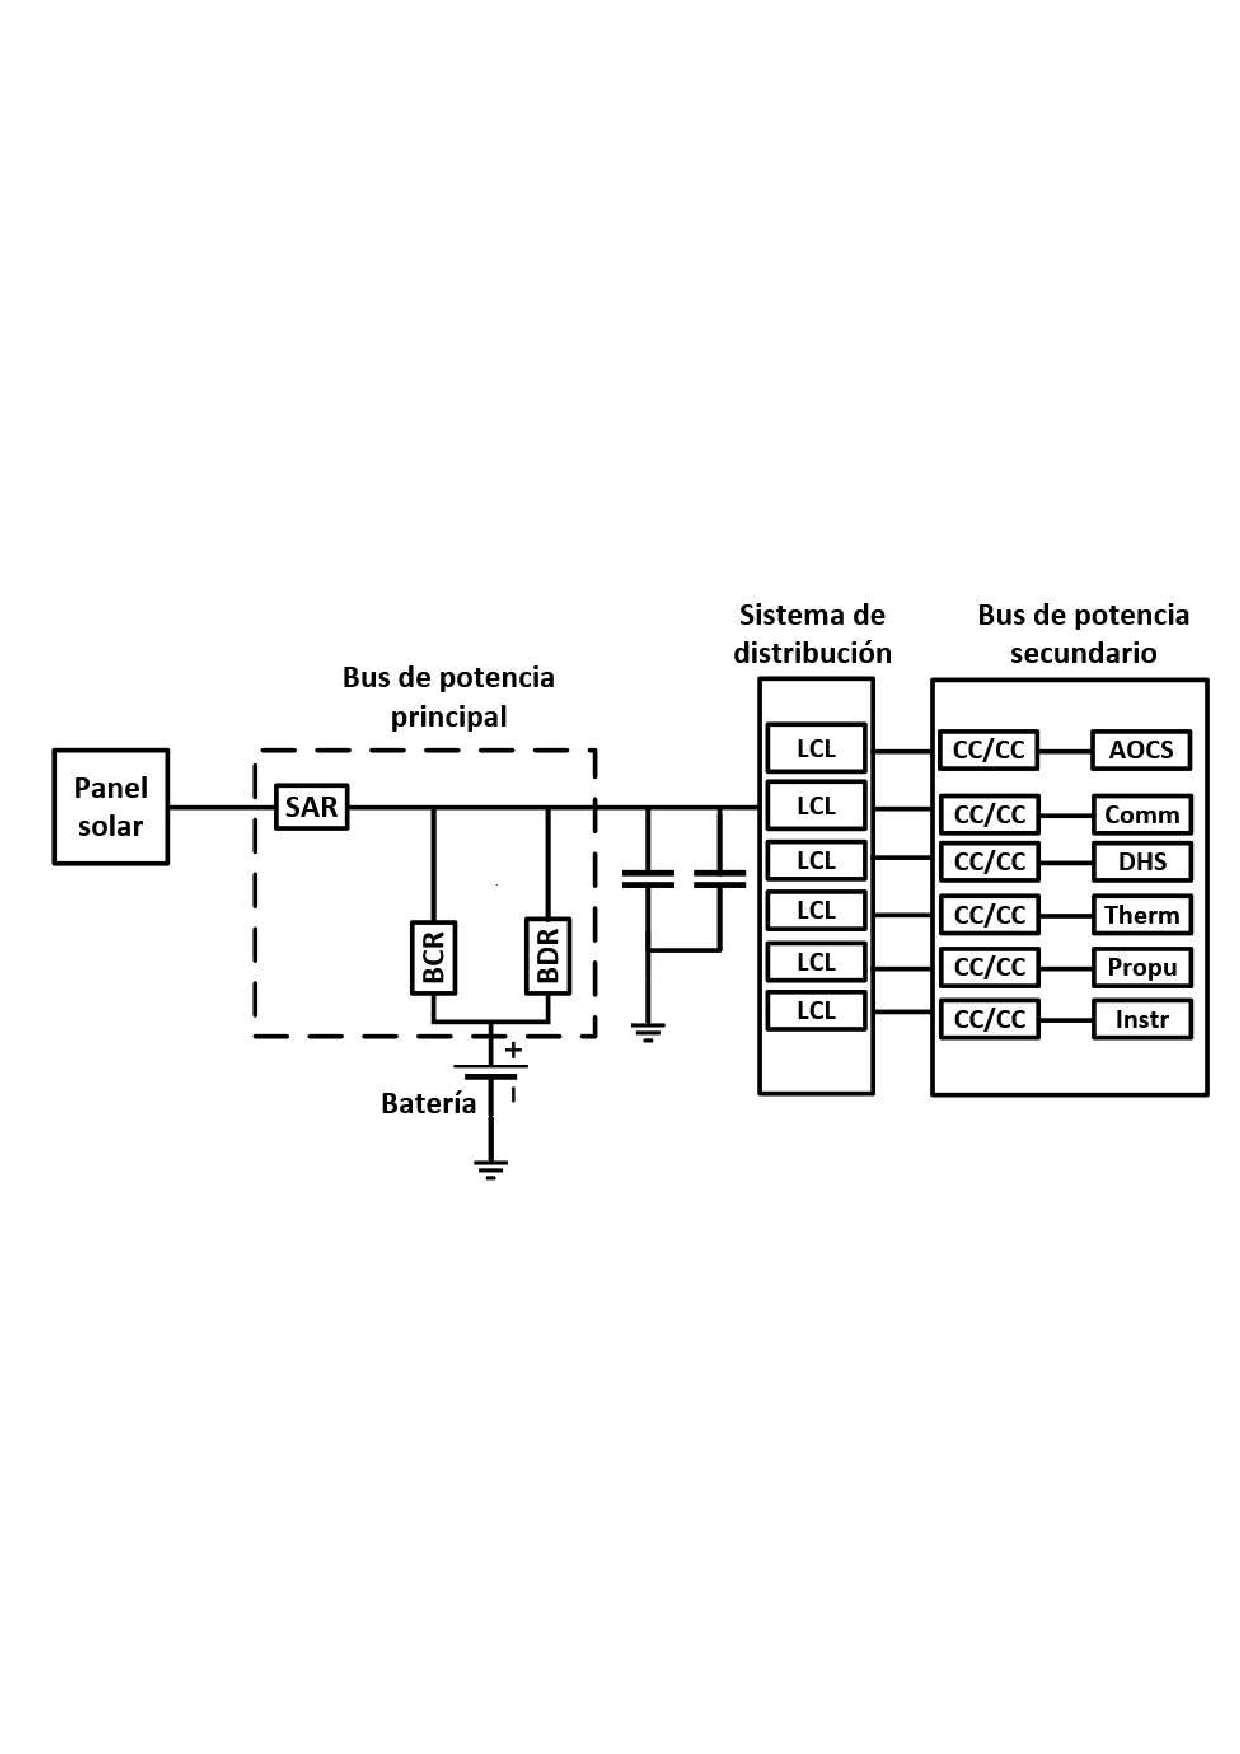
\includegraphics[width=\textwidth]{SistDistrib.pdf}\\
\footnotesize Un LCL por cada carga secundaria del satélite
}
\end{columns}



\note{
El LCL, Latching Current Limiter, es un dispositivo de protección de estado sólido que se coloca entre el bus principal de potencia de un satélite y cada carga secundaria. A diferencia de un fusible, no abre el circuito de forma instantánea: primero limita la corriente a un valor máximo prefijado y solo si el fallo persiste durante un tiempo determinado, el trip-off time, procede a desconectar la carga de forma enclavada, permitiendo rearmarla después por telecomando. Esta previsibilidad es lo que lo ha convertido en un estándar indispensable en el sector aeroespacial, donde no hay posibilidad de mantenimiento manual. El esquema de la derecha muestra un sistema de distribución de potencia típico de un satélite: del bus principal, alimentado por el panel solar y la batería, cuelga un sistema de distribución en el que cada carga secundaria (control de actitud, comunicaciones, propulsión, instrumentación...) está protegida por su propio LCL, de modo que un fallo en cualquiera de ellas nunca puede tumbar el bus completo.
}
\end{frame}

\begin{frame}
\transdissolve
\frametitle{El problema térmico del P-MOS lineal}

\begin{columns}
\column{0.5\textwidth}
\textbf{Topología clásica: P-MOS lineal}
\begin{itemize}
  \item<2-> Zona activa $\Rightarrow$ resistencia variable.
  \item<3-> Disipación: $P \approx V_\text{bus}\cdot I_\text{lim}$
  \item<4-> A 100 V con $I_\text{lim}=3{,}7$ A $\Rightarrow$ 370 W
  \item<5-> SOA excedida tras $7~ms$ 
\end{itemize}

\column{0.5\textwidth}
\centering
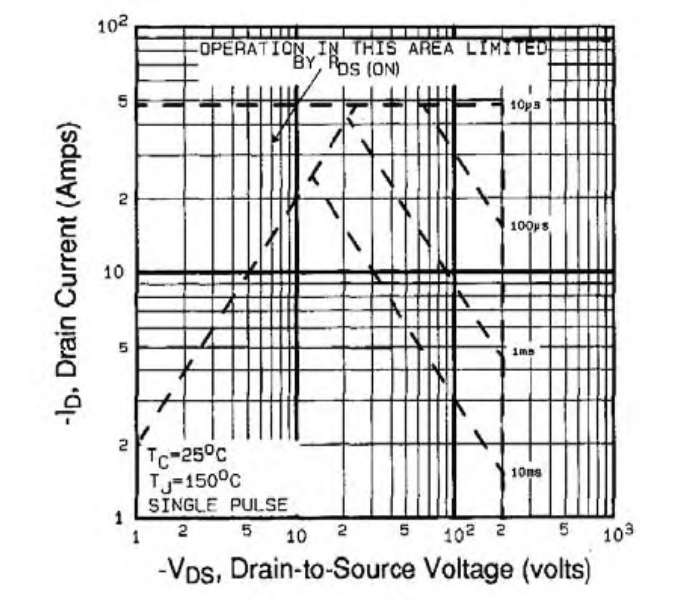
\includegraphics[width=\textwidth]{SOA.png}
\small SOA del P-MOS IRFP9240: a 100 V solo admite $<0{,}4$ A en continua.
\end{columns}

\note{
Las topologías tradicionales de LCL usan MOSFET de canal P operando en zona lineal durante la sobrecorriente: el transistor se comporta como una resistencia variable que absorbe toda la diferencia de tensión entre el bus y la carga. La potencia disipada es aproximadamente el producto de la tensión de bus por la corriente de limitación, así que al pasar de buses de 28 V a buses de 100 V esa potencia se dispara, en nuestro caso hasta unos 400 W. Esto es exactamente el problema que muestra esta gráfica de área de operación segura, la SOA, del fabricante Vishay para un P-MOS de canal P típico: a 100 V el dispositivo solo aguanta de forma continua corrientes inferiores a 0,4 amperios sin arriesgar la integridad del transistor. Aumentar el tiempo de trip-off con esta topología obligaría a usar semiconductores enormes y disipadores de calor muy grandes, lo cual es inviable en una aplicación espacial donde la masa es crítica.
}
\end{frame}

\begin{frame}
\transdissolve
\frametitle{La solución: N-MOS en conmutación}

\begin{columns}
\column{0.48\textwidth}
\textbf{Ventaja física del N-MOS}
\begin{itemize}
  \item<2-> \begin{equation*}
R_{\text{DS,ON}}\propto \frac{1}{\sigma} = \frac{1}{q (n\mu_n + p\mu_p)}
\label{eq:conductividad}
\end{equation*}
\vspace{-0.45cm}
\begin{equation*}
\begin{aligned}
\\ \mu_n &= 1350\ \text{cm}^2/\text{Vs} \\
\mu_p &= 480\ \text{cm}^2/\text{Vs}
\end{aligned}
\end{equation*}
%Movilidad de electrones $\approx 3\times$ la de los huecos $\Rightarrow$ $R_\text{DS(on)}$ $\approx 3\times$ menor.
  \item<3-> PWM $\Rightarrow P_\text{conmutadas} << P_\text{lineal}$
\end{itemize}

\column{0.48\textwidth}
\centering
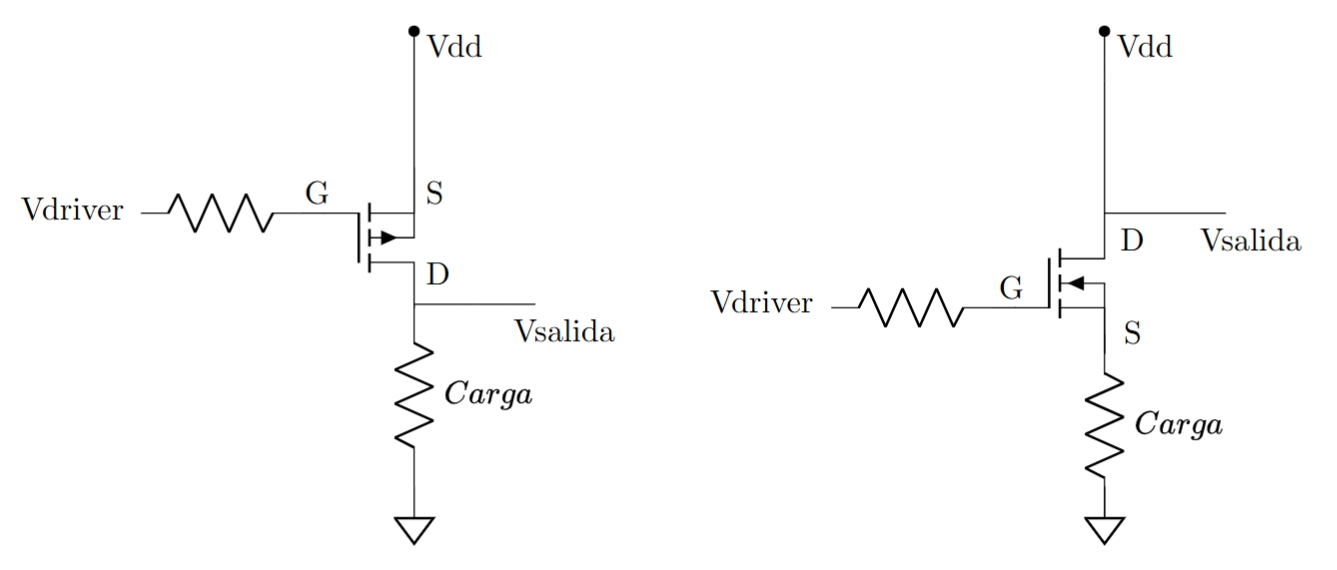
\includegraphics[width=0.9\textwidth]{HighSide.png}
\end{columns}

\vspace{0.35cm}
\begin{center}
\uncover<4->{\textbf{Dificultad:} disparo \textit{high-side} + $D=1$ $\Rightarrow$ alimentación flotante aislada.}
\end{center}

\note{
La solución que adopta este trabajo, siguiendo la línea de evolución de la industria desde los años 90, es sustituir el P-MOS lineal por un N-MOS operando en conmutación. La ventaja de partida es física: la movilidad de los electrones en el silicio es unas tres veces mayor que la de los huecos, así que un N-MOS tiene una resistencia de conducción unas tres veces menor que un P-MOS equivalente. Además, en conmutación el transistor solo pasa por dos estados, completamente abierto o completamente cerrado, minimizando las pérdidas instantáneas frente al modo lineal. El reto que introduce el N-MOS en configuración high-side es que la puerta necesita estar unos 15 voltios por encima de la fuente de forma permanente, y como en operación nominal el ciclo de trabajo es del 100\%, las técnicas clásicas de bootstrap no sirven porque no hay conmutación que recargue el condensador. Por eso este diseño incorpora una alimentación flotante mediante un convertidor DC-DC aislado dedicado.
}
\end{frame}

\begin{frame}
\transdissolve
\frametitle{Objetivos del TFG}

\textbf{Objetivo principal:}
\textit{Diseño}, \textit{simulación} y \textit{validación} experimental de un LCL en conmutación empleando un transistor N-MOS.

\pause
\vspace{0.3cm}
\textbf{Hitos metodológicos:}
\begin{itemize}
  \item Marco teórico: evolución P-MOS $\to$ N-MOS $\to$ N-MOS con materiales WBG.
  \pause
  \item Dimensionamiento teórico ($L_\text{min}$, $\Delta I_{\text{histéresis}}$, $t_\text{carga} \neq t_\text{descarga}$).
  \pause
  \item Modelado dinámico en \textbf{PSIM} con parásitos de componentes.
  \pause
  \item Diseño de PCB y validación. 
  \pause
  \item Metodología de escalado.
\end{itemize}

\note{
El objetivo principal del trabajo es diseñar, simular y validar experimentalmente un limitador de corriente de enclavamiento en conmutación basado en tecnología N-MOS, demostrando la mejora que supone frente a las topologías tradicionales de limitación lineal. Para llegar ahí se han seguido varios hitos: primero establecer el marco teórico de la evolución de los semiconductores de potencia; después dimensionar teóricamente el circuito, en particular la inductancia crítica, la banda de histéresis y el temporizador asimétrico; a continuación modelar el comportamiento dinámico en PSIM incorporando los parásitos reales de los componentes comerciales elegidos; construir y validar un prototipo físico en PCB comparando con las simulaciones; y finalmente desarrollar una metodología que permita escalar el diseño a otros niveles de tensión, corriente y tiempo de disparo.
}
\end{frame}

%==============================================================
\section{Diseño Teórico}
%==============================================================

\begin{frame}
\transdissolve
\frametitle{Especificaciones para el bus de 100 V}

\begin{columns}
\column{0.5\textwidth}
\small Sin clase ECSS-100 V estandarizada $\Rightarrow$ referencia más restrictiva de la clase de 28 V $\Rightarrow t_\text{trip-off} =1,5 ms$
\column{0.5\textwidth}
\centering
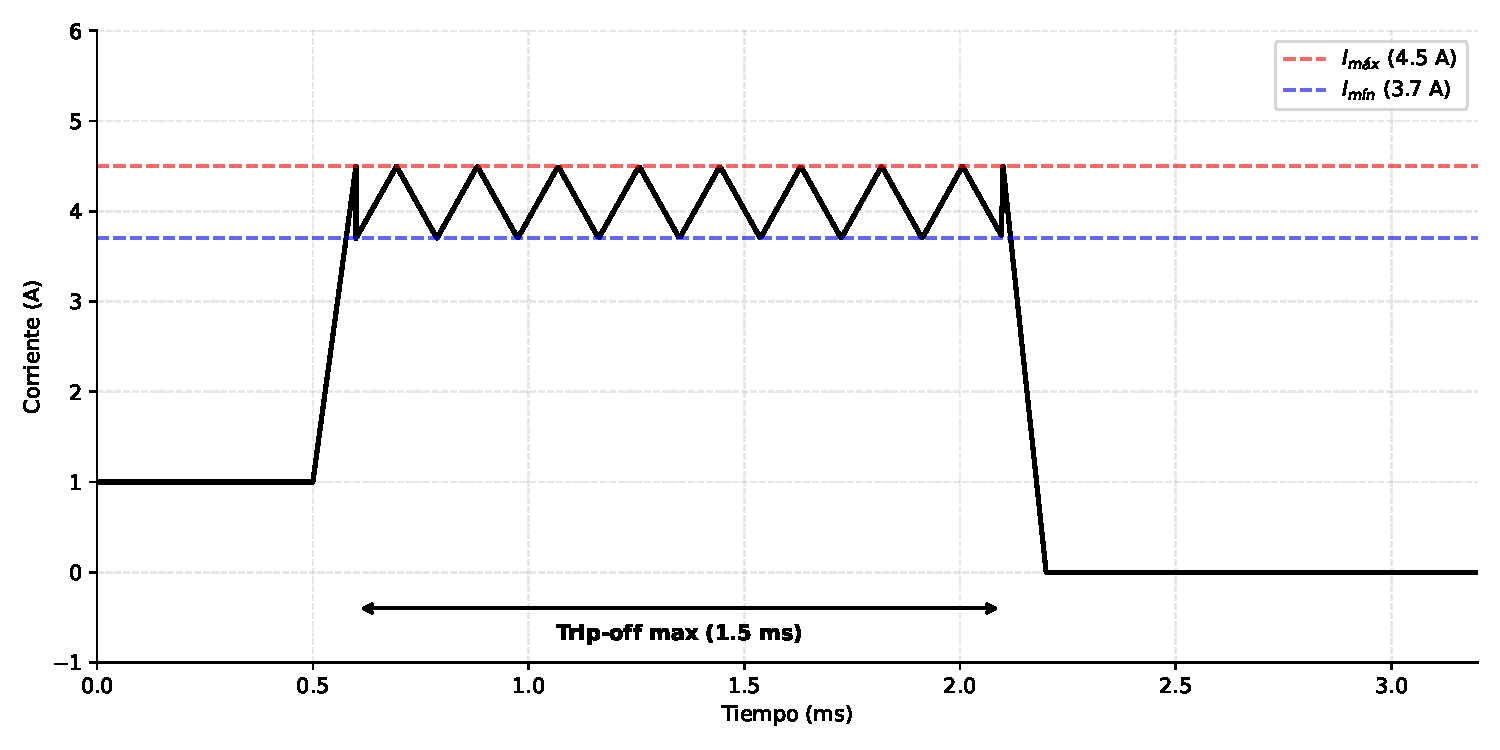
\includegraphics[width=\textwidth]{Histeresis.pdf}
\end{columns}
\pause
\vspace{-0.15cm}
\begin{table}
\centering
\resizebox{0.7\textwidth}{!}{
\begin{tabular}{ll}
\toprule
\textbf{Parámetro} & \textbf{Valor} \\
\midrule
Tensión de bus ($V_\text{bus}$) & 100 V \\
Corriente de limitación ($I_\text{lim}$) & 3,7 A \\
Banda de histéresis ($\Delta i$) & 0,8 A (3,7--4,5 A) \\
Tiempo de trip-off ($t_\text{trip}$) & 1,5 ms \\
\bottomrule
\end{tabular}
}
\end{table}

\note{
Los buses de 100 voltios todavía no tienen una clase estándar definida por la ECSS como sí existe para los buses de 28 voltios, así que hay libertad para elegir los parámetros pero también la obligación de justificarlos. Se ha elegido una corriente de limitación de 3,7 amperios, con una banda de histéresis de 0,8 amperios, de modo que el limitador conmuta entre 3,7 y 4,5 amperios. Para el tiempo de trip-off se ha adoptado el más restrictivo de las clases de 28 voltios, 1,5 milisegundos, precisamente porque al subir a 100 voltios la potencia disipada en el transistor durante la limitación es unas cuatro veces mayor que a 28 voltios, y conviene ser conservador. La gráfica de la derecha ilustra visualmente esa ventana de histéresis dentro de la que oscilará la corriente durante un fallo.
}
\end{frame}

\begin{frame}
\transdissolve
\frametitle{Arquitectura del limitador: Buck N-MOS \textit{high-side}}

\centering
\resizebox{!}{0.68\textheight}{
\begin{tikzpicture}[transform shape]
	% Paths, nodes and wires:
	\draw (11.373, 8.453) |- (11.333, 7.111);
	\draw (16.368, 4.614) -- (15.257, 4.614);
	\node[shape=rectangle, fill={rgb,255:red,255;green,255;blue,255}, draw={rgb,255:red,0;green,0;blue,0}, line width=1pt, minimum width=1.606cm, minimum height=1.08cm](N1) at (11.169, 6.669){} node[anchor=center] at (N1.text){$Driver$};
	\draw (19.111, 7.644) |- (19.111, 8.033);
	\draw (7.389, 8.928) to[american voltage source, l_={$Vbus$}, name=Vbus] (7.389, 8.178);
	\draw (9.056, 8.705) to[capacitor, /tikz/circuitikz/bipoles/length=0.980cm, l={$Cbus$}, label distance=-0.07cm] (9.056, 8.372);
	\node[nigfete, rotate=90](N2) at (11.103, 9.433){} node[anchor=south] at ([yshift=-0.09cm]N2.text){$NMOS$};
	\draw (12.75, 8.683) to[empty Schottky diode, /tikz/circuitikz/bipoles/length=0.840cm] (12.75, 9.183);
	\draw (14.889, 9.444) to[american inductor, i=$iL(t)$, current/distance=1] (17.222, 9.444);
	\draw (13.25, 9.433) to[american resistor, l_={$R shunt$}] (14.75, 9.433);
	\draw (17.556, 7.705) to[american resistor, l={$Carga$}] (17.556, 9.205);
	\draw (12.75, 9.433) -- (12.75, 9.183);
	\draw (12.29, 9.433) -- (13.25, 9.433);
	\draw (15.125, 9.433) -- (14.75, 9.433);
	\draw (16.875, 9.433) -| (17.556, 9.444) -| (17.556, 9.205);
	\draw (9.056, 8.933) -| (9.056, 9.433) -- (9.556, 9.433);
	\node[ground] at (9.056, 7.705){};
	\node[ground] at (12.75, 7.683){};
	\node[ground] at (17.556, 7.705){};
	\node[ground] at (7.389, 7.678){};
	\draw (7.389, 8.178) -| (7.389, 7.678);
	\draw (9.056, 9.433) -| (7.389, 9.428);
	\draw (7.389, 9.428) -| (7.389, 8.928);
	\draw (9.056, 8.372) -| (9.056, 7.372);
	\draw (12.75, 8.683) -| (12.75, 7.683);
	\draw (19.111, 9.034) to[american voltage source, l={$Vcc$}] (19.111, 8.283);
	\draw (19.111, 7.783) -- (19.111, 8.283);
	\node[shape=rectangle, minimum width=1.801cm, minimum height=1.076cm] at (20.444, 7.556){} node[anchor=north west, align=left, text width=1.427cm, inner sep=5.8pt] at (19.526, 8.111){Masa Control};
	\node[ocirc] at (19.111, 7.783){};
	\draw (13.183, 10.193) -| (12.75, 9.433);
	\node[ocirc] at (13.235, 10.193){};
	\node[shape=rectangle, minimum width=2.737cm, minimum height=0.455cm] at (14.569, 10.193){} node[anchor=center, align=center, text width=2.561cm, inner sep=3pt] at (14.569, 10.193){Masa Control};
	\draw (19.111, 9.534) -| (19.111, 9.034);
	\node[ocirc, xscale=-1, yscale=-1](N3) at (19.111, 9.534){} node[anchor=north] at ([yshift=0.52cm]N3.text){$Vcc$};
	\node[sground] at (19.111, 7.644){};
	\node[ieeestd and port, rotate=90, xscale=0.72, yscale=0.72] at (11.333, 5.333){};
	\draw (17.205, 3.486) |- (17.705, 3.486);
	\node[ocirc, rotate=90] at (17.205, 3.486){};
	\node[shape=rectangle, minimum width=1.525cm, minimum height=0.665cm] at (16.425, 3.486){} node[anchor=north west, align=left, text width=1.137cm, inner sep=6pt] at (15.644, 3.836){Vsense};
	\draw (15, 8.211) -| (15, 8.711);
	\draw (15, 8.156) -- (15, 8.656);
	\node[ocirc, xscale=-1, yscale=-1] at (15, 8.156){};
	\node[shape=rectangle, minimum width=1.165cm, minimum height=0.865cm] at (15.044, 7.883){} node[anchor=center, align=center, text width=0.988cm, inner sep=3pt] at (15.044, 7.883){Vmeas};
	\node[shape=rectangle, minimum width=1.703cm, minimum height=0.865cm] at (14.833, 2.392){} node[anchor=center, align=center, text width=1.526cm, inner sep=3pt] at (14.833, 2.392){Vmeas};
	\node[shape=rectangle, fill={rgb,255:red,255;green,255;blue,255}, draw={rgb,255:red,0;green,0;blue,0}, line width=1pt, minimum width=3.076cm, minimum height=1.076cm] at (17.979, 4.392){} node[anchor=center, align=center, text width=2.688cm, inner sep=6pt] at (17.979, 4.392){Control por Histéresis\\};
	\node[shape=rectangle, fill={rgb,255:red,255;green,255;blue,255}, draw={rgb,255:red,0;green,0;blue,0}, line width=1pt, minimum width=3.131cm, minimum height=1.076cm] at (13.563, 4.392){} node[anchor=center, align=center, text width=2.743cm, inner sep=6pt] at (13.563, 4.392){Biestable\\};
	\node[shape=rectangle, minimum width=1.187cm, minimum height=0.374cm] at (15.757, 4.965){} node[anchor=north, align=center, text width=0.799cm, inner sep=6pt] at (15.757, 5.17){Set};
	\node[shape=rectangle, minimum width=1.187cm, minimum height=0.352cm] at (15.757, 4.343){} node[anchor=north, align=center, text width=0.799cm, inner sep=6pt] at (15.757, 4.536){Reset};
	\draw[-latex] (16.313, 4.614) -- (15.146, 4.614);
	\draw[-latex] (16.368, 3.993) -- (15.146, 3.993);
	\draw (11.535, 4.554) -- (11.535, 4.392) -- (11.979, 4.392);
	\node[shape=rectangle, minimum width=1.187cm, minimum height=0.52cm] at (11.651, 4.233){} node[anchor=north, align=center, text width=0.799cm, inner sep=6pt] at (11.651, 4.51){Q};
	\draw[-latex] (18.007, 2.948) -| (17.979, 3.836);
	\node[shape=rectangle, fill={rgb,255:red,255;green,255;blue,255}, draw={rgb,255:red,0;green,0;blue,0}, line width=1pt, minimum width=3.131cm, minimum height=1.076cm] at (7.874, 4.399){} node[anchor=center, align=center, text width=2.743cm, inner sep=6pt] at (7.874, 4.399){Temporizador\\};
	\draw (10.702, 4.392) -| (11.132, 4.554);
	\node[shape=rectangle, minimum width=1.742cm, minimum height=0.512cm] at (10.243, 4.281){} node[anchor=north, align=center, text width=1.354cm, inner sep=6pt] at (10.243, 4.554){Shutdown};
	\draw (10.702, 4.392) -| (9.457, 4.399);
	\node[shape=rectangle, minimum width=1.631cm, minimum height=0.665cm] at (8.096, 3.083){} node[anchor=north west, align=left, text width=1.243cm, inner sep=6pt] at (7.263, 3.433){Vsense};
	\draw (15.702, 2.392) |- (16.202, 2.392);
	\node[ocirc, rotate=90] at (15.702, 2.392){};
	\draw (8.096, 3.383) -| (8.096, 3.883);
	\node[ocirc, xscale=-1, yscale=-1] at (8.096, 3.383){};
	\draw (15, 8.656) -| (15, 9.433);
	\node[shape=rectangle, minimum width=1.165cm, minimum height=0.514cm] at (16.289, 9.202){} node[anchor=center, align=center, text width=0.988cm, inner sep=3pt] at (16.289, 9.202){L};
	\node[shape=rectangle, minimum width=1.165cm, minimum height=0.865cm] at (12.956, 8.539){} node[anchor=center, align=center, text width=0.988cm, inner sep=3pt] at (12.956, 8.539){D};
	\draw (6.651, 5.455) -| (6.651, 4.955);
	\node[ocirc, xscale=-1, yscale=-1](N4) at (6.651, 5.455){} node[anchor=north] at ([yshift=0.52cm]N4.text){$Vcc$};
	\draw (13.563, 5.448) -| (13.563, 4.947);
	\node[ocirc, xscale=-1, yscale=-1](N5) at (13.563, 5.448){} node[anchor=north] at ([yshift=0.52cm]N5.text){$Vcc$};
	\draw (19.313, 3.448) -| (19.313, 2.948);
	\node[ocirc, xscale=-1, yscale=-1](N6) at (19.313, 3.448){} node[anchor=west] at ([xshift=0.09cm]N6.north east){$Vcc$};
	\node[sground] at (19.318, 1.899){};
	\node[sground] at (13.563, 3.836){};
	\node[sground] at (6.651, 3.844){};
	\node[sground] at (18.535, 3.836){};
	\draw (18.535, 5.448) -| (18.535, 4.948);
	\node[ocirc, xscale=-1, yscale=-1](N7) at (18.535, 5.448){} node[anchor=west] at ([xshift=0.09cm]N7.north east){$Vcc$};
	\draw (17.705, 3.486) -| (17.986, 3.503);
	\draw (10.54, 7.733) -| (10.54, 7.233);
	\node[ocirc, xscale=-1, yscale=-1](N8) at (10.54, 7.733){} node[anchor=north] at ([yshift=0.52cm]N8.text){$Vcc$};
	\node[sground] at (10.54, 6.122){};
	\node[shape=rectangle, fill={rgb,255:red,255;green,255;blue,255}, draw={rgb,255:red,0;green,0;blue,0}, line width=1pt, minimum width=3.465cm, minimum height=1.076cm] at (17.952, 2.392){} node[anchor=center, align=center, text width=3.077cm, inner sep=6pt] at (17.952, 2.392){Sensor Corriente\\(Ganancia K)};
	\draw (12.29, 9.433) -- (11.873, 9.433);
	\draw (9.556, 9.433) -- (10.333, 9.433);
	\draw (9.056, 8.933) -- (9.056, 8.705);
	\node[shape=rectangle, draw={rgb,255:red,255;green,0;blue,0}, line width=0.6pt, dash pattern={on 2.4pt off 1.2pt}, minimum width=0.757cm, minimum height=0.646cm] at (7.389, 7.222){};
	\node[shape=rectangle, draw={rgb,255:red,255;green,0;blue,0}, line width=0.6pt, dash pattern={on 2.4pt off 1.2pt}, minimum width=0.757cm, minimum height=0.646cm] at (9.056, 7.222){};
	\node[shape=rectangle, draw={rgb,255:red,255;green,0;blue,0}, line width=0.6pt, dash pattern={on 2.4pt off 1.2pt}, minimum width=0.757cm, minimum height=0.646cm] at (12.778, 7.222){};
	\node[shape=rectangle, draw={rgb,255:red,255;green,0;blue,0}, line width=0.6pt, dash pattern={on 2.4pt off 1.2pt}, minimum width=0.757cm, minimum height=0.646cm] at (17.556, 7.222){};
	\node[shape=rectangle, draw={rgb,255:red,0;green,0;blue,255}, line width=0.6pt, dash pattern={on 2.4pt off 1.2pt}, minimum width=0.757cm, minimum height=0.646cm] at (6.667, 3.333){};
	\node[shape=rectangle, draw={rgb,255:red,0;green,0;blue,255}, line width=0.6pt, dash pattern={on 2.4pt off 1.2pt}, minimum width=0.757cm, minimum height=0.646cm] at (13.556, 3.333){};
	\node[shape=rectangle, draw={rgb,255:red,0;green,0;blue,255}, line width=0.6pt, dash pattern={on 2.4pt off 1.2pt}, minimum width=0.757cm, minimum height=0.646cm] at (18.556, 3.333){};
	\node[shape=rectangle, draw={rgb,255:red,0;green,0;blue,255}, line width=0.6pt, dash pattern={on 2.4pt off 1.2pt}, minimum width=0.757cm, minimum height=0.646cm] at (19.333, 1.333){};
	\node[shape=rectangle, draw={rgb,255:red,0;green,0;blue,255}, line width=0.6pt, dash pattern={on 2.4pt off 1.2pt}, minimum width=0.757cm, minimum height=0.646cm] at (19.167, 7.111){};
\end{tikzpicture}
}

\pause
\vspace{0.2cm}
\small La bobina controla dinámicamente la corriente. \\Diodo de libre circulación (Schottky) en el nodo de conmutación.

\note{
Este es el esquema real del convertidor. El N-MOS actúa como interruptor en serie con la carga, en topología de convertidor reductor o buck, y está en el lado de alta tensión, high-side. A diferencia de un buck convencional, no hay condensador de salida: se deja que sea únicamente la bobina la que controle de forma dinámica la corriente, porque un condensador de salida enmascararía las variaciones de corriente que el sistema necesita detectar. El driver excita la puerta del N-MOS y recibe su energía de una alimentación flotante referenciada a la fuente del transistor, no a la masa del sistema (masa control). La resistencia Rshunt mide la corriente que fluye hacia la carga; esa señal, Vsense, se acondiciona y alimenta el bloque de histéresis y el temporizador, cuyas salidas gobiernan un biestable que, a través de la puerta lógica y el driver, cierra el lazo de control. También hay un diodo de libre circulación Schottky en el nudo de conmutación para dar salida a la corriente de la bobina cuando el N-MOS está abierto.
}
\end{frame}

\begin{frame}
\transdissolve
\frametitle{Sensado y acondicionamiento de la corriente}

\begin{itemize}
  \item $R_\text{shunt} = 22\text{ m}\Omega$: \textit{trade-off} pérdidas, integridad de señal y caída de tensión.
\end{itemize}

\pause
\vspace{-0.2cm}
{\footnotesize
\begin{equation*}
R_\text{shunt}
\begin{cases}
  \ \gg 22\text{ m}\Omega: & \uparrow P_\text{shunt}=I^{2}R \ \text{ y } \ \downarrow V_\text{carga}\quad (1\,\Omega \Rightarrow 3{,}7\text{ V de caída}) \\[3pt]
  \ \ll 22\text{ m}\Omega: & V_\text{sense} \approx  V_\text{EMI} \Rightarrow \text{disparos falsos}
\end{cases}
\end{equation*}
}
\vspace{-0.25cm}

\pause
\begin{itemize}
  \item Caída por $I_\text{lim}$: $V_\text{sense} = I_\text{lim}\cdot R_\text{shunt} = 81{,}4\text{ mV}$ ($\approx 0{,}081$\,\% de $V_\text{bus}$).
  \pause
  \item OPAMPS en cascada con LPF:
\end{itemize}

\pause
\begin{columns}[c]
\column{0.52\textwidth}
\centering
\resizebox{\linewidth}{!}{%
\begin{tikzpicture}[transform shape]
	% Paths, nodes and wires:
	\node[op amp, xscale=0.52, yscale=0.52] at (6.25, 7.25){};
	\node[op amp, xscale=0.52, yscale=0.52] at (9.619, 6.995){};
	\draw (5.25, 8.5) to[american resistor, l={$R2$}] (7, 8.5);
	\draw (8.75, 8.25) to[american resistor, l={$R4$}] (10.5, 8.25);
	\draw (3, 8.5) to[american resistor, l={$R1$}] (4.75, 8.5);
	\draw (6.869, 7.25) to[american resistor, l={$R3$}] (8.619, 7.25);
	\draw (8.619, 7.25) -- (9, 7.25);
	\draw (8.75, 8.25) -- (8.75, 7.25);
	\draw (10.5, 8.25) |- (10.238, 6.995);
	\draw (7, 8.5) -- (7, 7.25);
	\draw (5.25, 8.5) -| (5.25, 7.5) -| (5.631, 7.505);
	\draw (4.75, 7) -| (5.631, 6.995);
	\node[shape=rectangle, minimum width=1.703cm, minimum height=0.865cm] at (4, 7){} node[anchor=center, align=center, text width=1.526cm, inner sep=3pt] at (4, 7){Vmeas};
	\draw (5.5, 9.5) to[capacitor, /tikz/circuitikz/bipoles/length=0.700cm, l={$C1$}] (6.75, 9.5);
	\draw (6.75, 9.5) -| (7, 8.5);
	\draw (5.5, 9.5) -- (5.25, 9.5) -- (5.25, 8.5);
	\draw (4.75, 8.5) -- (5.25, 8.5);
	\draw (9, 9.25) to[capacitor, /tikz/circuitikz/bipoles/length=0.700cm, l={$C2$}] (10.25, 9.25);
	\draw (10.25, 9.25) -| (10.5, 8.25);
	\draw (9, 9.25) -- (8.75, 9.25) -- (8.75, 8.25);
	\node[shape=rectangle, minimum width=1.525cm, minimum height=0.665cm] at (11.5, 7){} node[anchor=north west, align=left, text width=1.137cm, inner sep=6pt] at (10.72, 7.35){Vsense};
	\node[sground] at (2.75, 8.25){};
	\draw (2.75, 8.25) -| (2.75, 8.5) -- (3, 8.5);
	\node[sground] at (8.75, 6.5){};
	\draw (8.75, 6.5) -| (8.75, 6.75) -- (9, 6.75);
	\node[shape=rectangle, minimum width=3.715cm, minimum height=1.215cm] at (7.75, 5.75){} node[anchor=north west, align=left, text width=3.341cm, inner sep=5.8pt] at (5.875, 6.375){Masa Control};
	\node[shape=rectangle, minimum width=3.59cm, minimum height=1.367cm] at (1.813, 7.451){} node[anchor=north west, align=left, text width=3.216cm, inner sep=5.8pt] at (0, 8.153){Masa Control};
	\draw (10.75, 7) -- (10.5, 7);
\end{tikzpicture}%
}

\column{0.46\textwidth}
\centering
\begin{equation*}
  G = \left(1+\frac{R_2}{R_1}\right)\cdot\left(-\frac{R_4}{R_3}\right) \approx -25\ \text{V/V}
\end{equation*}

\vspace{0.3cm}
\pause
\small $81{,}4\text{ mV} \xrightarrow{\times(-25)} 2{,}035\text{ V}$ \\(referencia usada por histéresis y temporizador)
\end{columns}

\note{
Para que el lazo de control sepa cuándo conmutar el MOSFET hace falta medir la corriente. Se usa una resistencia de sensado de solo 22 miliohmios, y ese valor sale de un compromiso que se ve bien en los dos extremos. Si la resistencia fuese mucho mayor, las pérdidas por efecto Joule crecerían y, sobre todo, la caída de tensión dejaría de ser despreciable: con un ohmio tendríamos 3,7 voltios de caída, es decir, 96,3 voltios en la carga en lugar de los 99,9 que tenemos ahora. Si fuese mucho menor, la tensión medida quedaría al nivel del ruido de conmutación y de las interferencias electromagnéticas, con riesgo de disparos falsos. Con 22 miliohmios la caída a la corriente de limitación es solo un 0,081 por ciento del bus. La señal resultante, unos 81,4 milivoltios a la corriente de limitación, es demasiado pequeña para trabajar cómodamente, así que se amplifica con dos amplificadores operacionales en cascada con una ganancia total de aproximadamente menos 25 voltios por voltio, que además incorporan filtros paso bajo para eliminar el ruido de alta frecuencia de la conmutación. El resultado son 2,035 voltios, que es la referencia que usarán tanto el bloque de histéresis como el de temporización.
}
\end{frame}

\begin{frame}
\transdissolve
\frametitle{Lógica de Control: Máquina de Estados}

{\scriptsize
$t < t_{trip-off} \Rightarrow$ Temporizador $=1$\\
$I < I_{max} \Rightarrow$ Biestable $=1$\par}
\vspace{-0.7cm}

\begin{figure}
\centering
\resizebox{0.68\textwidth}{!}{
\begin{tikzpicture}[transform shape]
	% Paths, nodes and wires:
	\node[shape=ellipse, draw, line width=1pt, minimum width=5.879cm, minimum height=3.629cm] at (4.207, 6.125){};
	\draw[line width=0.7pt] (7.039, 6.625) -- (1.414, 6.625);
	\node[shape=rectangle, minimum width=5.5cm, minimum height=0.75cm] at (4.164, 7.375){} node[anchor=north, align=center, text width=5.147cm, inner sep=5pt] at (4.164, 7.75){ESTADO 0: \\NOMINAL};
	\node[shape=rectangle, minimum width=4.25cm, minimum height=1.375cm] at (2.914, 5.625){} node[anchor=north, align=center, text width=3.897cm, inner sep=5pt] at (2.914, 6.313){Histéresis = 1\\Biestable = 1};
	\node[shape=rectangle, minimum width=0.625cm, minimum height=0.75cm] at (4.602, 5.875){} node[anchor=north west, align=left, text width=0.385cm, inner sep=3.4pt] at (4.289, 6.25){\huge \}};
	\node[shape=rectangle, minimum width=4.25cm, minimum height=1.375cm] at (5.833, 5.354){} node[anchor=north, align=center, text width=3.897cm, inner sep=5pt] at (5.833, 6.042){$V_{gs}=+15~V$};
	\node[shape=ellipse, draw, line width=1pt, minimum width=5.879cm, minimum height=3.629cm] at (4.23, 0.5){};
	\draw[line width=0.7pt] (7.062, 1) -- (1.438, 1);
	\node[shape=rectangle, minimum width=5.5cm, minimum height=0.75cm] at (4.25, 1.75){} node[anchor=north, align=center, text width=5.147cm, inner sep=5pt] at (4.25, 2.125){ESTADO 1:\\LIMITACIÓN (N-MOS ON)};
	\node[shape=rectangle, minimum width=4.25cm, minimum height=1.375cm] at (2.938, -0){} node[anchor=north, align=center, text width=3.897cm, inner sep=5pt] at (2.938, 0.687){Histéresis = 1\\Biestable = 1};
	\node[shape=rectangle, minimum width=0.625cm, minimum height=0.75cm] at (4.625, 0.25){} node[anchor=north west, align=left, text width=0.385cm, inner sep=3.4pt] at (4.312, 0.625){\huge \}};
	\node[shape=rectangle, minimum width=4.25cm, minimum height=1.375cm] at (5.938, -0.188){} node[anchor=north, align=center, text width=3.897cm, inner sep=5pt] at (5.938, 0.5){$V_{gs}=+15~V$};
	\node[shape=ellipse, draw, line width=1pt, minimum width=5.879cm, minimum height=3.629cm] at (16.091, 0.6){};
	\draw[line width=0.7pt] (18.923, 1.1) -- (13.298, 1.1);
	\node[shape=rectangle, minimum width=5.5cm, minimum height=0.75cm] at (16.111, 1.85){} node[anchor=north, align=center, text width=5.147cm, inner sep=5pt] at (16.111, 2.225){ESTADO 2:\\LIMITACIÓN (N-MOS OFF)};
	\node[shape=rectangle, minimum width=4.25cm, minimum height=1.375cm] at (14.798, 0.1){} node[anchor=north, align=center, text width=3.897cm, inner sep=5pt] at (14.798, 0.788){Histéresis = 0\\Biestable = 1};
	\node[shape=rectangle, minimum width=0.625cm, minimum height=0.75cm] at (16.486, 0.35){} node[anchor=north west, align=left, text width=0.385cm, inner sep=3.4pt] at (16.173, 0.725){\huge \}};
	\node[shape=rectangle, minimum width=4.25cm, minimum height=1.375cm] at (17.625, -0.187){} node[anchor=north, align=center, text width=3.897cm, inner sep=5pt] at (17.625, 0.5){$V_{gs}=0~V$};
	\node[shape=ellipse, draw, line width=1pt, minimum width=5.879cm, minimum height=3.629cm] at (16.043, 6.25){};
	\draw[line width=0.7pt] (18.875, 6.75) -- (13.25, 6.75);
	\node[shape=rectangle, minimum width=5.5cm, minimum height=0.75cm] at (16.063, 7.5){} node[anchor=north, align=center, text width=5.147cm, inner sep=5pt] at (16.063, 7.875){ESTADO 3:\\ENCLAVAMIENTO};
	\node[shape=rectangle, minimum width=4.25cm, minimum height=1.375cm] at (14.75, 5.75){} node[anchor=north, align=center, text width=3.897cm, inner sep=5pt] at (14.75, 6.437){Histéresis = -\\Biestable = 0};
	\node[shape=rectangle, minimum width=0.625cm, minimum height=0.75cm] at (16.438, 6){} node[anchor=north west, align=left, text width=0.385cm, inner sep=3.4pt] at (16.125, 6.375){\huge \}};
	\node[shape=rectangle, minimum width=4.25cm, minimum height=1.375cm] at (17.625, 5.5){} node[anchor=north, align=center, text width=3.897cm, inner sep=5pt] at (17.625, 6.187){$V_{gs}=0~V$};
	\draw[line width=1.8pt, -latex] (2.125, 4.875) -- (2.139, 1.795);
	\draw[line width=1.8pt, -latex] (6.321, 1.795) -- (6.298, 4.829);
	\draw[line width=1.8pt, -latex] (13.086, 6.25) |- (7.164, 6.125);
	\node[shape=rectangle, minimum width=5.965cm, minimum height=0.465cm] at (10.25, 6.75){} node[anchor=north, align=center, text width=5.577cm, inner sep=6pt] at (10.25, 7){\Large Reinicio manual};
	\node[shape=rectangle, minimum width=3.298cm, minimum height=0.465cm] at (3.667, 3.417){} node[anchor=north west, align=left, text width=2.91cm, inner sep=6pt] at (2, 3.667){\Large $I \geq I_{lim}$};
	\node[shape=rectangle, draw, draw opacity=0.02, line width=1pt, minimum width=3.298cm, minimum height=0.465cm] at (8, 3.333){} node[anchor=north west, align=left, text width=2.903cm, inner sep=6.1pt] at (6.333, 3.583){\Large $I <I_{lim}$};
	\node[shape=rectangle, minimum width=5.965cm, minimum height=0.798cm] at (10.167, 0.083){} node[anchor=north, align=center, text width=5.577cm, inner sep=6pt] at (10.167, 0.5){\Large $I \geq I_{max} $ , $t < t_{trip-off}$};
	\node[shape=rectangle, minimum width=6.131cm, minimum height=0.798cm] at (10.2, -2.817){} node[anchor=north, align=center, text width=5.743cm, inner sep=6pt] at (10.2, -2.4){\Large $I \leq I_{min} $ , $t < t_{trip-off}$};
	\draw[line width=1.8pt, -latex] (7.167, 0.5) -- (13.167, 0.5);
	\draw[line width=1.8pt, -latex] (16.091, 2.432) -- (16.125, 4.5);
	\draw[line width=1.8pt, -latex] (16.2, -1.2) -- (16.2, -2.4) -- (4.2, -2.4) -- (4.23, -1.332);
	\node[shape=rectangle, minimum width=3.798cm, minimum height=0.798cm] at (17.583, 3.417){} node[anchor=north, align=center, text width=3.41cm, inner sep=6pt] at (17.583, 3.833){\Large $t \geq t_{trip-off}$};
	\draw[line width=1.8pt, -latex] (7.062, 1) -- (13.952, 4.954);
	\node[shape=rectangle, minimum width=3.798cm, minimum height=0.798cm] at (12.417, 3){} node[anchor=north, align=center, text width=3.41cm, inner sep=6pt] at (12.417, 3.417){\Large $t \geq t_{trip-off}$};
	\node[shape=circle, draw={rgb,255:red,0;green,0;blue,255}, line width=1pt, minimum width=2.465cm] at (10.116, 9.866){};
	\path[draw={rgb,255:red,0;green,0;blue,255}, line width=1pt] (8.866, 9.866) -- (11.366, 9.866);
	\node[shape=rectangle, minimum width=2.465cm, minimum height=0.465cm] at (10.116, 10.366){} node[anchor=north, align=center, text width=2.077cm, inner sep=6pt] at (10.116, 10.616){\textcolor{rgb,255:red,0;green,0;blue,255}{ESTADO}};
	\node[shape=rectangle, minimum width=2.465cm, minimum height=0.465cm] at (10.116, 9.366){} node[anchor=north, align=center, text width=2.077cm, inner sep=6pt] at (10.116, 9.616){\textcolor{rgb,255:red,0;green,0;blue,255}{SALIDA}};
	\path[draw={rgb,255:red,0;green,0;blue,255}, line width=1.8pt, -latex] (11.366, 9.866) -- (13.366, 9.866);
	\node[shape=rectangle, minimum width=5.965cm, minimum height=0.465cm] at (12.616, 10.366){} node[anchor=north, align=center, text width=5.577cm, inner sep=6pt] at (12.616, 10.616){\textcolor{rgb,255:red,0;green,0;blue,255}{ENTRADA}};
\end{tikzpicture}
}
\end{figure}

\note{
Esta máquina de estados resume toda la lógica de control. En el estado 0, funcionamiento nominal, la corriente está por debajo del límite y el driver mantiene la puerta a más 15 voltios de forma constante. Si la corriente alcanza el límite de limitación se pasa al estado 1, limitación con el N-MOS encendido, y si supera el límite superior de histéresis se pasa al estado 2, limitación con el N-MOS apagado; el circuito alterna entre estos dos estados conmutando a la frecuencia de diseño mientras el temporizador cuenta el tiempo de trip-off. Si la corriente vuelve a bajar del límite inferior antes de que se cumpla ese tiempo, se regresa al estado nominal. Pero si el temporizador alcanza el tiempo de trip-off, 1,5 milisegundos, sin que la corriente haya bajado, el sistema pasa al estado 3, enclavamiento, con la puerta a 0 voltios y la carga aislada, y solo sale de ahí mediante un reinicio manual.
}
\end{frame}

\begin{frame}
\transdissolve
\frametitle{Dimensionado clave: inductancia y frecuencia}

\begin{table}
\centering
\resizebox{\textwidth}{!}{
\begin{tabular}{lll}
\toprule
\textbf{Criterio (ECSS-E-ST-20-20C)} & \textbf{$L_\text{min}$} & \textbf{Comentario} \\
\midrule
Req. 5.4.1.1.1a/b (cortocircuito repentino) & 3,116 $\mu$H & Limita $I_\text{max}=10$ A \\
Req. 5.4.1.1.1e (carga máx. de entrada 1 mC) & 1,7 $\mu$H & Peor caso $V_\text{out}=V_\text{bus}/2$ \\
Req. 5.2.3.1a (\textit{overshoot} tras histéresis) & \textbf{42,85 $\boldsymbol{\mu}$H} & El más restrictivo \\
\bottomrule
\end{tabular}
}
\end{table}

\pause
\vspace{0.3cm}
\centering
{\Large $L$ = \textbf{68 $\boldsymbol{\mu}$H} (valor comercial) $\Rightarrow$ $f_\text{sw}$ = \textbf{614,98 kHz}}

\note{
La bobina es el componente más determinante del diseño porque fija a la vez la frecuencia de conmutación y la capacidad de frenar la subida de corriente ante un cortocircuito. Se han evaluado tres requisitos de la norma ECSS-E-ST-20-20C adaptados a nuestro caso, cada uno dando una inductancia mínima distinta: 3,116 microhenrios por el requisito de cortocircuito repentino, 1,7 microhenrios por el requisito de carga máxima de entrada, y 42,85 microhenrios por el requisito de que el pico tras el rebase de histéresis no sea destructivo, siendo este último el más restrictivo y el que fija el valor mínimo real. A partir de ahí, y buscando un valor comercial estándar con un margen razonable, se ha elegido una bobina de 68 microhenrios, que resulta en una frecuencia de conmutación teórica de 614,98 kilohercios para el peor caso de ciclo de trabajo del 50 por ciento.
}
\end{frame}

\begin{frame}
\transdissolve
\frametitle{Temporizador asimétrico y memoria térmica}

\begin{columns}
  
\column{0.5\textwidth}
\centering

\resizebox{0.7\textwidth}{!}{
\begin{tikzpicture}[transform shape]
	% Paths, nodes and wires:
	\draw (30.5, 11.5) to[empty diode, /tikz/circuitikz/bipoles/length=0.700cm] (31.2, 11.5);
	\draw (33, 11.5) to[american resistor, l={$R_{descarga}$}] (31.119, 11.5);
	\draw (32.5, 12.25) to[empty diode, /tikz/circuitikz/bipoles/length=0.700cm] (31.25, 12.25);
	\draw (32.5, 12.25) -| (33, 11.5);
	\draw (31.281, 12.25) -- (30.581, 12.25) -| (30.5, 11.45);
	\draw (30.506, 11.3) to[capacitor, /tikz/circuitikz/bipoles/length=0.700cm, l_={$C_{timer}$}] (30.506, 10.2);
	\node[sground] at (30.5, 10.5){};
	\draw (33, 14.4) -| (33, 13.9);
	\node[ocirc, xscale=-1, yscale=-1](N1) at (33, 14.4){} node[anchor=west] at ([xshift=0.09cm]N1.north east){$Vcc$};
	\draw (33, 12.25) to[american resistor, l={$R_{carga}$}] (33, 13.9);
	\draw (30.506, 11.55) -- (30.506, 11.3);
\end{tikzpicture}}\\
\small Red RC \textbf{asimétrica} de carga/descarga
\column{0.5\textwidth}
\textbf{Carga (sobrecorriente):}
\begin{itemize}
  \item $C_\text{timer}=100\text{ nF}$, $R_3=26{,}1\text{ k}\Omega$
  \pause
  \item $\tau_\text{carga}$ ajustada a $t_\text{trip}=1{,}5\text{ ms}$
\end{itemize}
\pause
\textbf{Descarga (memoria térmica):}
\begin{itemize}
  \item $R_\text{descarga}=100\text{ k}\Omega >> R_\text{carga}$
  \pause
  \item $t_\text{descarga}=63{,}05\text{ ms}$
\end{itemize}

\end{columns}

\note{
El temporizador cuenta cuánto tiempo lleva el sistema limitando corriente y, si supera 1,5 milisegundos, ordena el enclavamiento. Para conseguir ese tiempo se carga un condensador de 100 nanofaradios a través de una resistencia de 26,1 kilohmios hasta un voltaje de referencia de 2,035 voltios. Pero la red es asimétrica: la descarga se hace a través de una resistencia mucho mayor, de 100 kilohmios, lo que da una constante de descarga de 63 milisegundos, muy superior a la de carga. Esto dota al sistema de memoria térmica: si el transistor sufre dos sobrecorrientes muy seguidas en el tiempo, el condensador no ha tenido tiempo de descargarse del todo tras la primera, así que en la segunda alcanza el umbral de disparo mucho antes, protegiendo al N-MOS de un sobrecalentamiento acumulado aunque cada fallo individual sea corto.
}
\end{frame}

%==============================================================
\section{Componentes y Simulación PSIM}
%==============================================================

\begin{frame}
\transdissolve
\frametitle{Componentes comerciales seleccionados}

\begin{table}
\centering
\resizebox{\textwidth}{!}{
\begin{tabular}{lll}
\toprule
\textbf{Bloque} & \textbf{Componente} & \textbf{Motivo clave} \\
\midrule
MOSFET de potencia & IRFB4020PbF & $Q_G=18\text{ nC}$: conmutación antes que conducción; 200 V ($+100\%$) \\
Driver de puerta & UCC27511AQDBVRQ1 & Salida dividida 4 A / 8 A (anti-Miller), retardo 13 ns \\
Diodo de libre circulación & STPSC6H065B-TR (SiC) & $Q_\text{rr}\approx 0$: sin falsos disparos; 650 V ($+550\%$) \\
Comparador histéresis & LM319AM/NOPB & Retardo 70 ns y salida en colector abierto \\
Comparador temporizador & LM393BIDR & 200 $\mu$A/canal; 1 $\mu$s despreciable frente a 1,5 ms \\
Bobina de potencia & WE-HCI 74435586800 & Hilo plano, saturación suave, apantallada (EMI) \\
OPAMP de sensado & OPA2836QDGKRQ1 & 205 MHz y 560 V/$\mu$s, entrada \textit{negative-rail} \\
Alim. flotante & TMA 1515S + L78L05CD13TR & Aislamiento galvánico +15 V; LDO de bajo ruido +5 V \\
\bottomrule
\end{tabular}
}
\end{table}

\note{
La selección de componentes prioriza la disponibilidad comercial en distribuidores como Mouser o DigiKey y la velocidad de respuesta frente a la calificación espacial, coherente con el enfoque de prototipo de laboratorio. El MOSFET IRFB4020PbF de Infineon se elige precisamente por su compromiso: tiene una resistencia en conducción relativamente alta, 80 miliohmios, porque lo que se ha priorizado es la respuesta dinámica, es decir, una carga de puerta baja de 18 nanoculombios para conmutar rápido y con pocas pérdidas; además da un margen de tensión del cien por cien respecto al bus. Es de silicio y no de carburo de silicio porque para un prototipo inicial el precio y la complejidad del disparo, que exigiría alimentación simétrica, no se justifican. El driver UCC27511A aporta una corriente de pico asimétrica, hasta 4 amperios al encender y 8 al apagar, lo que además evita el reencendido por efecto Miller, con salida dividida para ajustar por separado las resistencias de encendido y apagado y solo 13 nanosegundos de retardo. El diodo de libre circulación sí es de carburo de silicio: al ser Schottky su carga de recuperación inversa es prácticamente nula, lo que evita el pico de corriente inversa que dispararía las pérdidas de conmutación y podría provocar falsos disparos del limitador, y sus 650 voltios suponen un margen del 550 por ciento que hace innecesario un snubber. Para los comparadores se ha diferenciado velocidad y consumo: el LM319 de alta velocidad para la histéresis, con 70 nanosegundos de retardo y salida en colector abierto que ataca directamente al driver sin lógica intermedia; y el LM393B para el temporizador, con un consumo de apenas 200 microamperios por canal, ya que su retardo de 1 microsegundo es despreciable frente a los 1,5 milisegundos que debe contar, y usar aquí un comparador rápido sería un sobrediseño. La bobina Würth Elektronik usa hilo plano para mitigar el efecto pelicular y el de proximidad a 615 kilohercios, núcleo de saturación suave que evita que la pendiente de corriente se dispare antes de que actúen los comparadores, y apantallamiento metálico, clave cuando la señal de medida son apenas 81 milivoltios. El amplificador OPA2836 aporta 205 megahercios de ancho de banda y 560 voltios por microsegundo de slew rate, junto con la arquitectura de entrada negative-rail necesaria para amplificar señales muy cercanas a la masa local; es lo que permite cerrar el tiempo de sensado en 171,4 nanosegundos. Y la pareja TMA1515S más L78L05 genera la alimentación flotante: el convertidor DC/DC con aislamiento galvánico da los 15 voltios referidos a la fuente del MOSFET, y el regulador lineal baja a 5 voltios con poco ruido, evitando meter más interferencia electromagnética en el lazo de control.
}
\end{frame}

\begin{frame}
\transdissolve
\frametitle{Esquema eléctrico en KiCad: potencia}

\centering
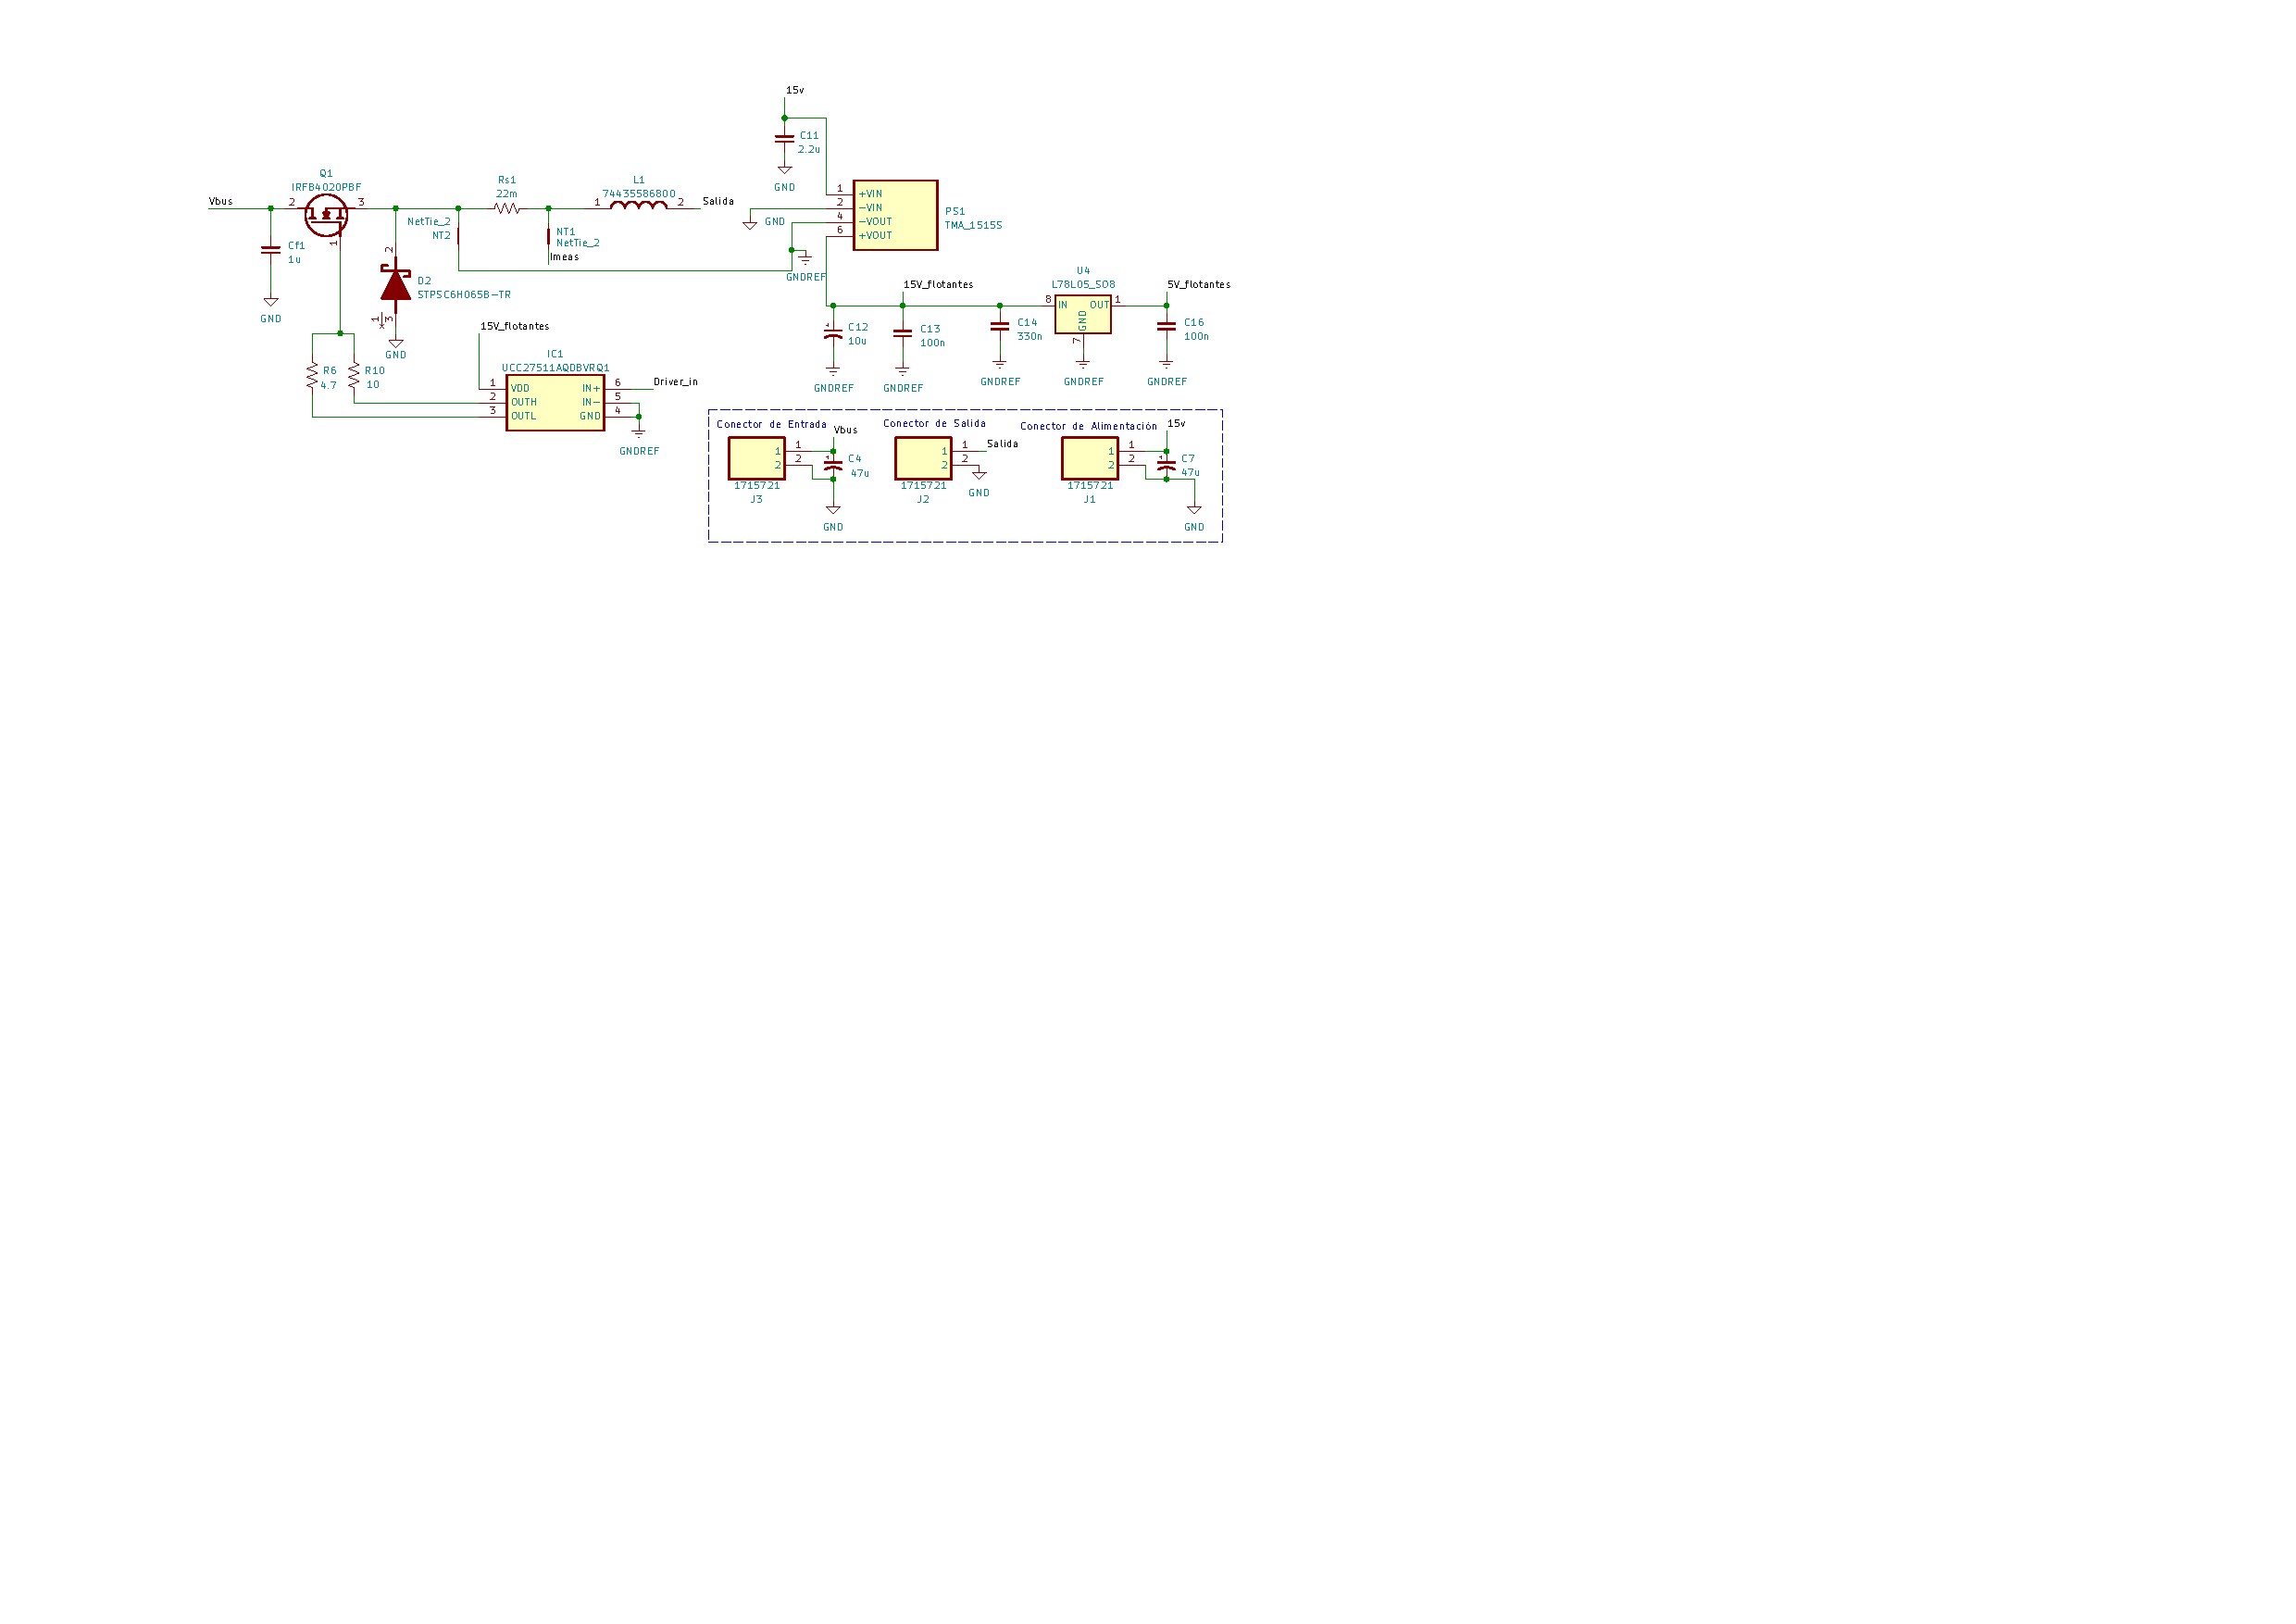
\includegraphics[width=0.92\textwidth]{PKicadSch.pdf}\\
\small Etapa de potencia y alimentación flotante

\note{
Este es el bloque de potencia real diseñado en KiCad: el conector de entrada del bus, el MOSFET Q1 disparado por el driver IC1 con resistencias diferenciadas de encendido y apagado, y el convertidor TMA1515S que genera la alimentación flotante de 15 voltios junto al regulador lineal que baja a 5 voltios. También se usan componentes NetTie para implementar un conexionado Kelvin y así separar la ruta de potencia de la ruta de medida de tensión.
}
\end{frame}

\begin{frame}
\transdissolve
\frametitle{Esquema eléctrico en KiCad: histéresis}

\centering
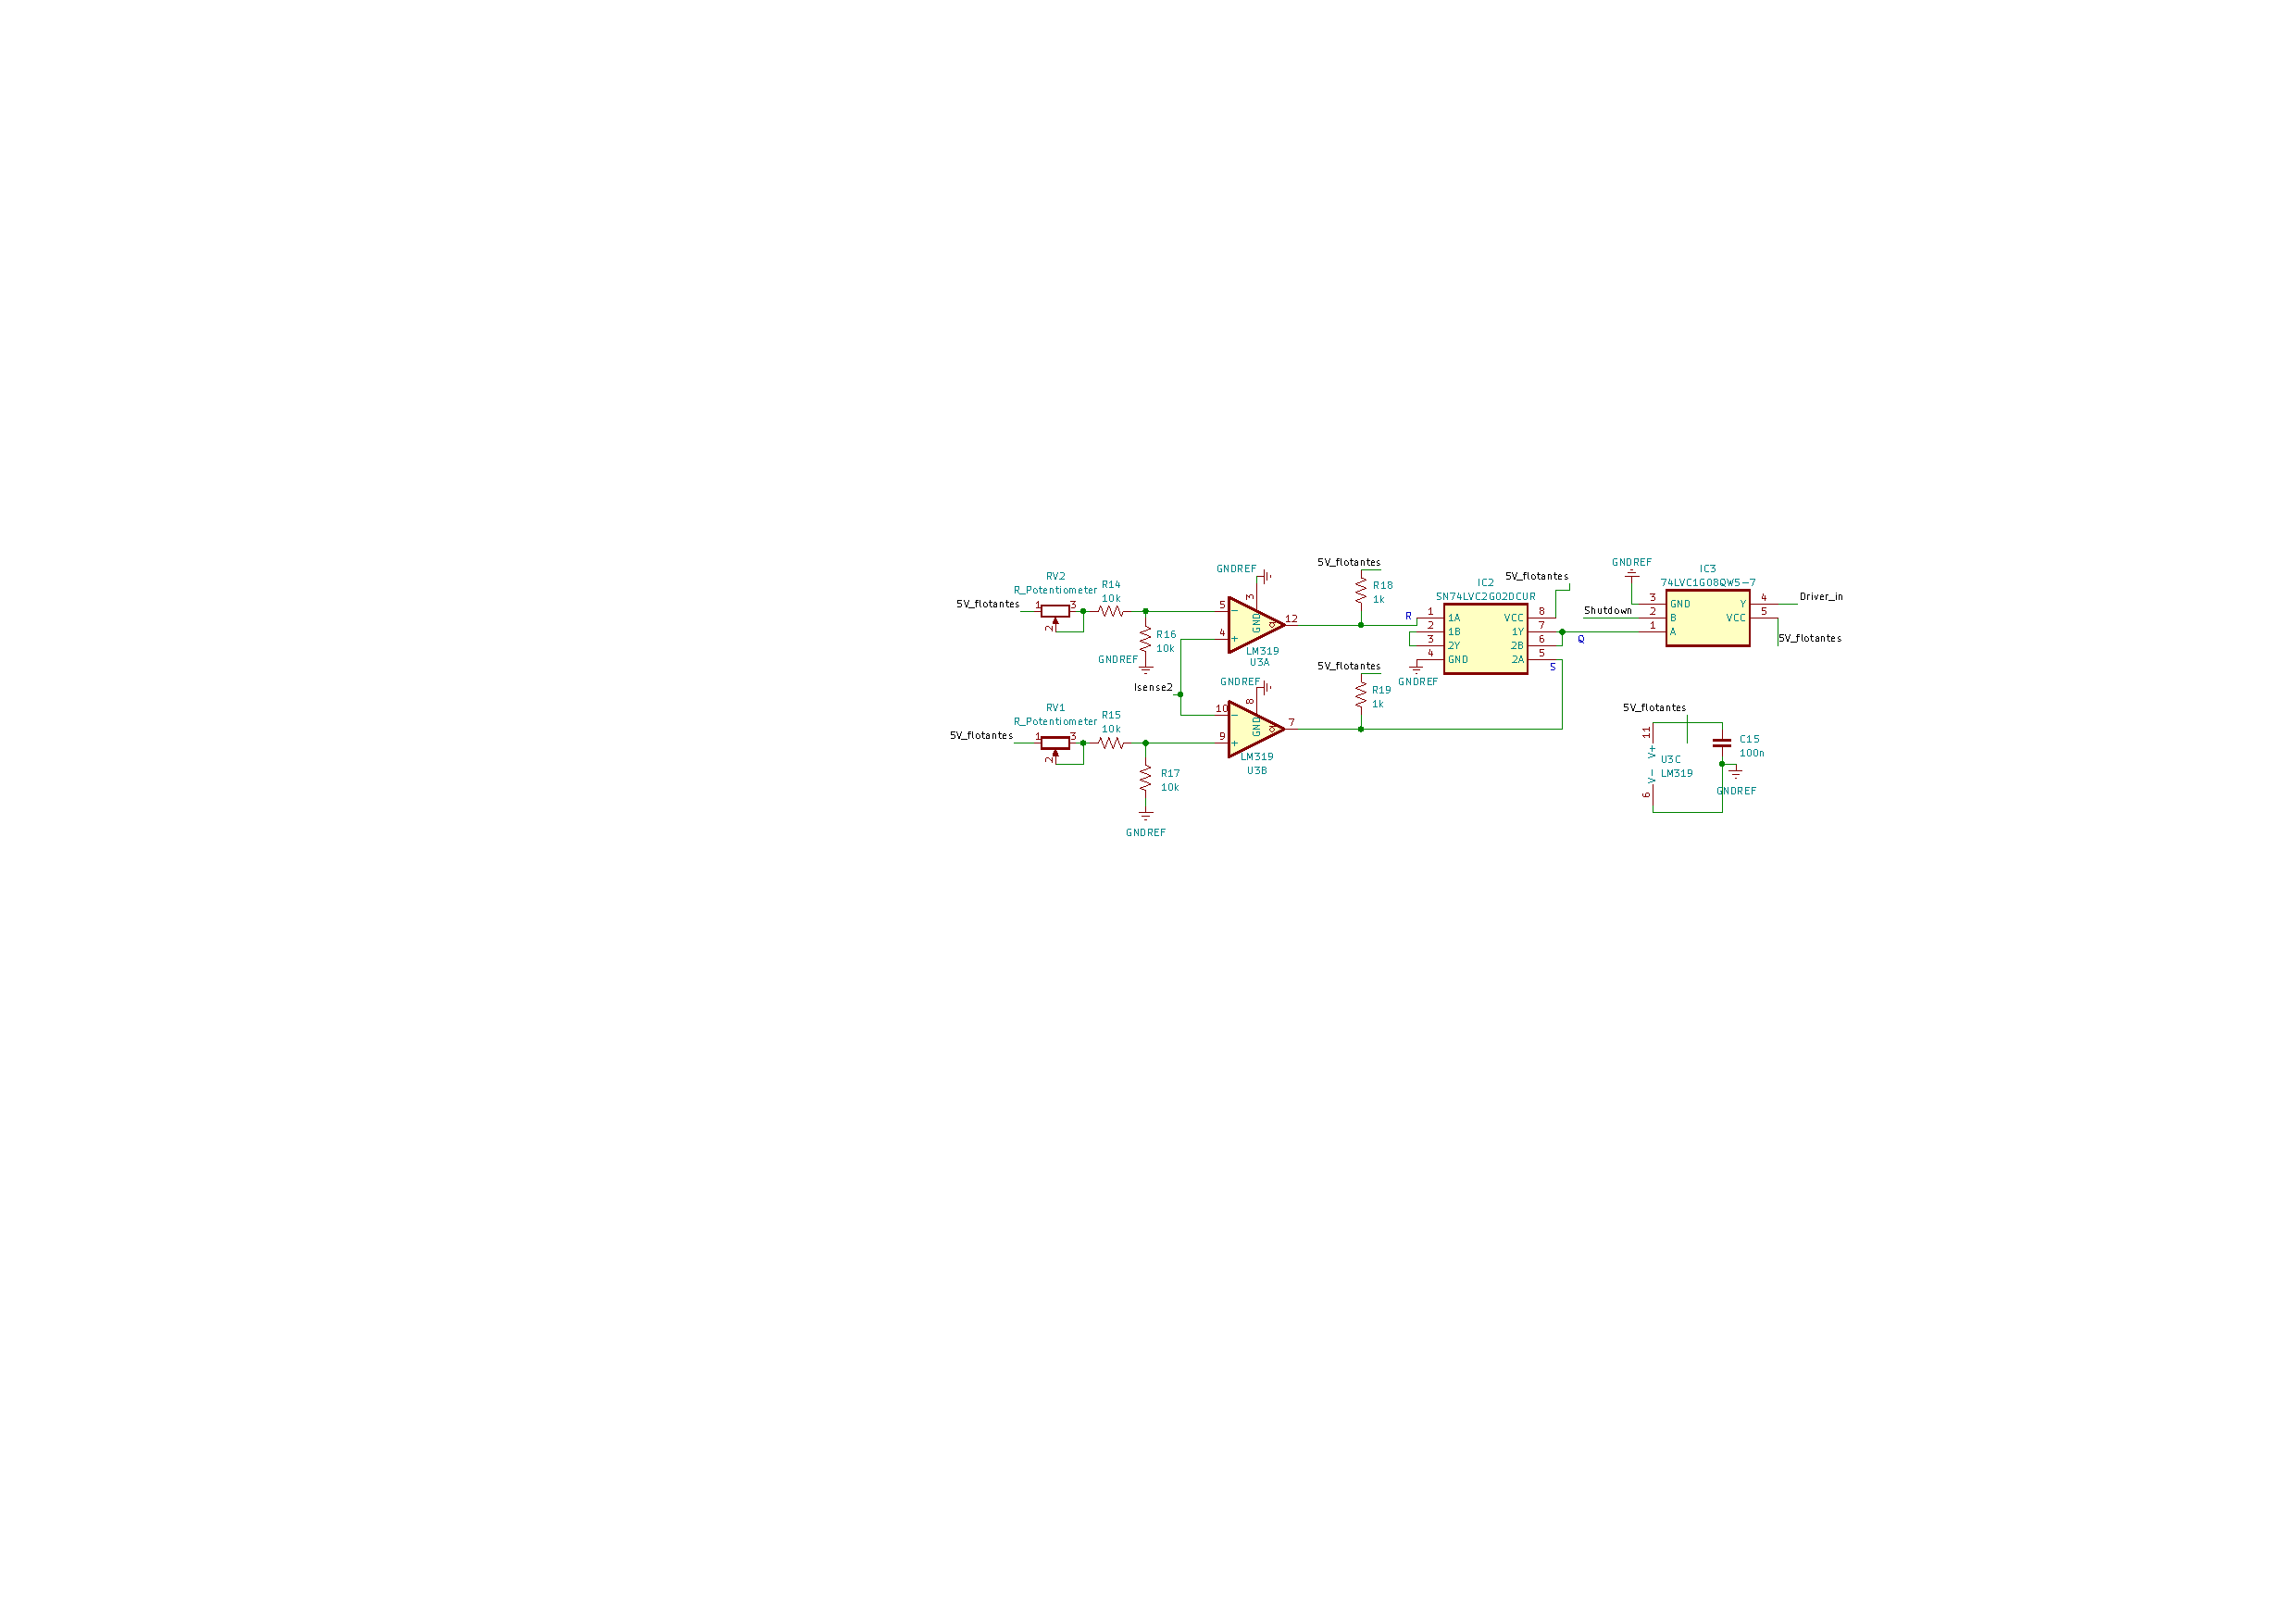
\includegraphics[width=0.92\textwidth]{HisteresisKicadSch.pdf}\\
\small Histéresis y enclavamiento (biestable RS)

\note{
El bloque de histéresis: dos comparadores LM319 en colector abierto comparan la señal amplificada de corriente contra los límites superior e inferior, ajustables mediante los potenciómetros RV1 y RV2, y su salida alimenta un biestable RS construido con puertas NOR que memoriza el estado del limitador.
}
\end{frame}

\begin{frame}
\transdissolve
\frametitle{Esquema eléctrico en KiCad: acondicionamiento}

\centering
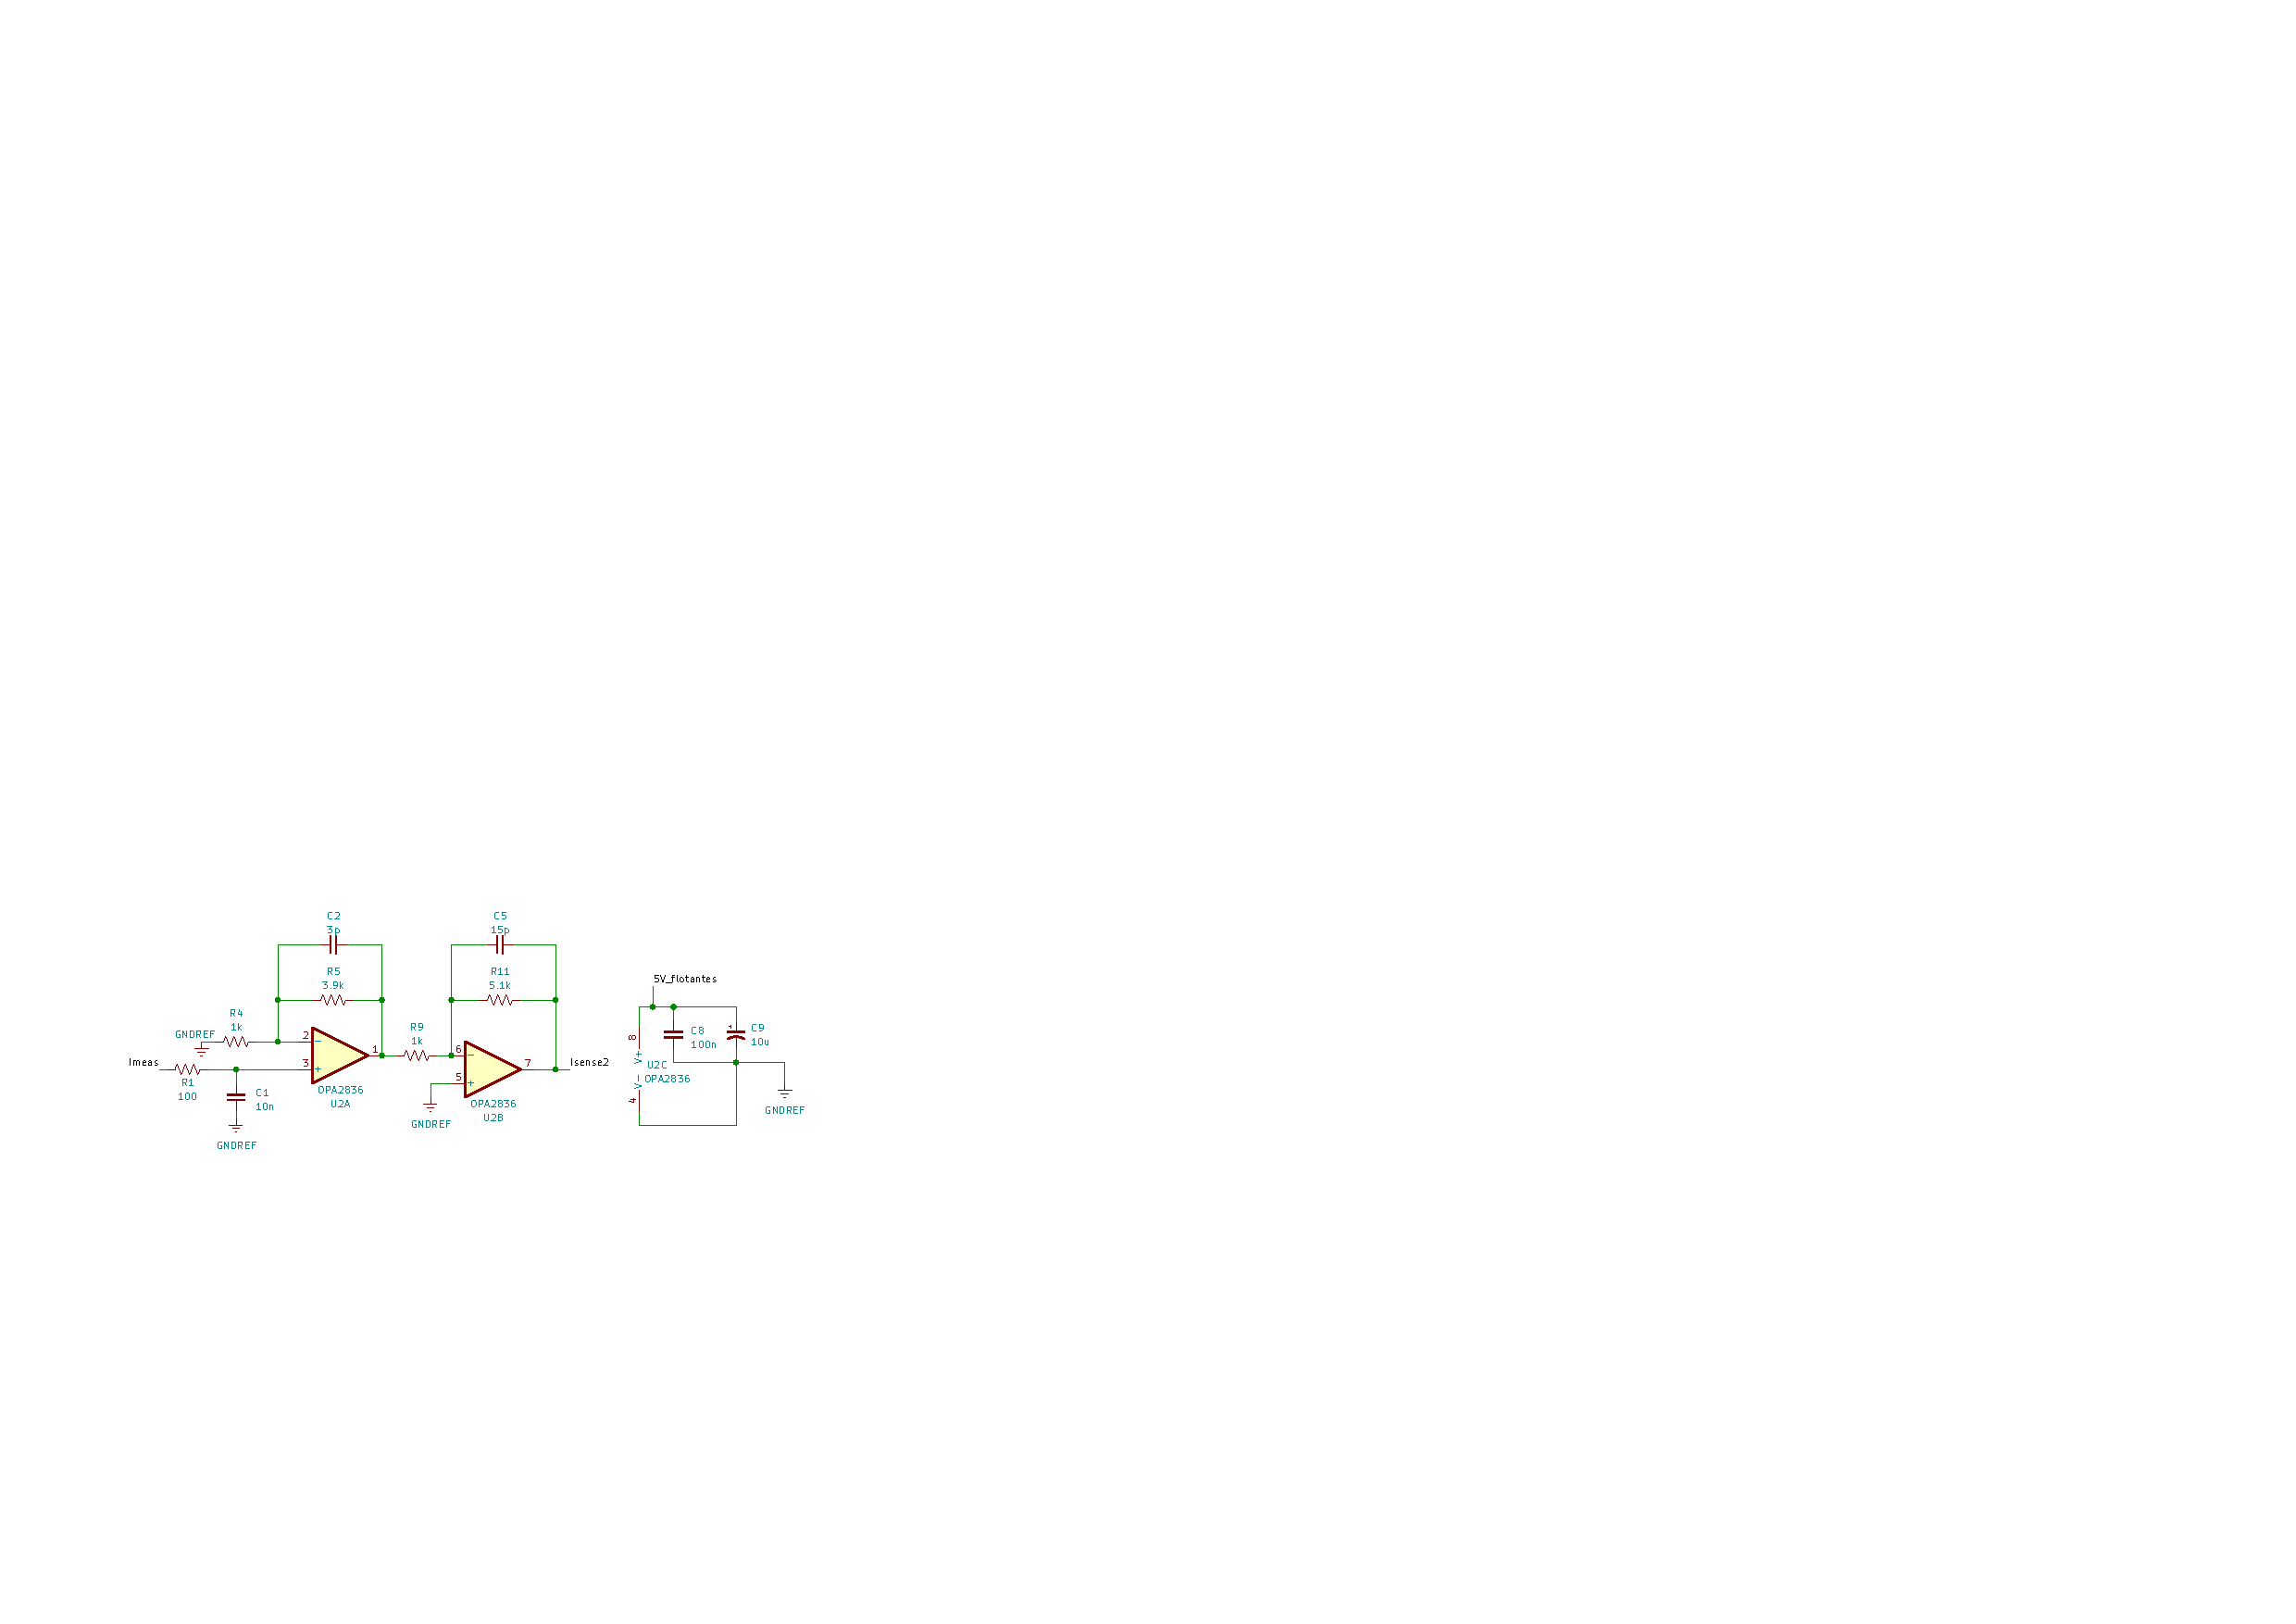
\includegraphics[width=0.92\textwidth]{AcondicionamientoKicadSch.pdf}\\
\small Acondicionamiento de la señal de corriente

\note{
El bloque de acondicionamiento: la señal Imeas procedente de la resistencia de sensado pasa por la red de amplificadores operacionales con ganancia menos 25, con tres filtros paso bajo en cascada para dar estabilidad y limpiar el ruido de conmutación antes de entregar la señal Isense2 a los bloques de histéresis y temporización.
}
\end{frame}

\begin{frame}
\transdissolve
\frametitle{Esquema eléctrico en KiCad: temporizador}

\centering
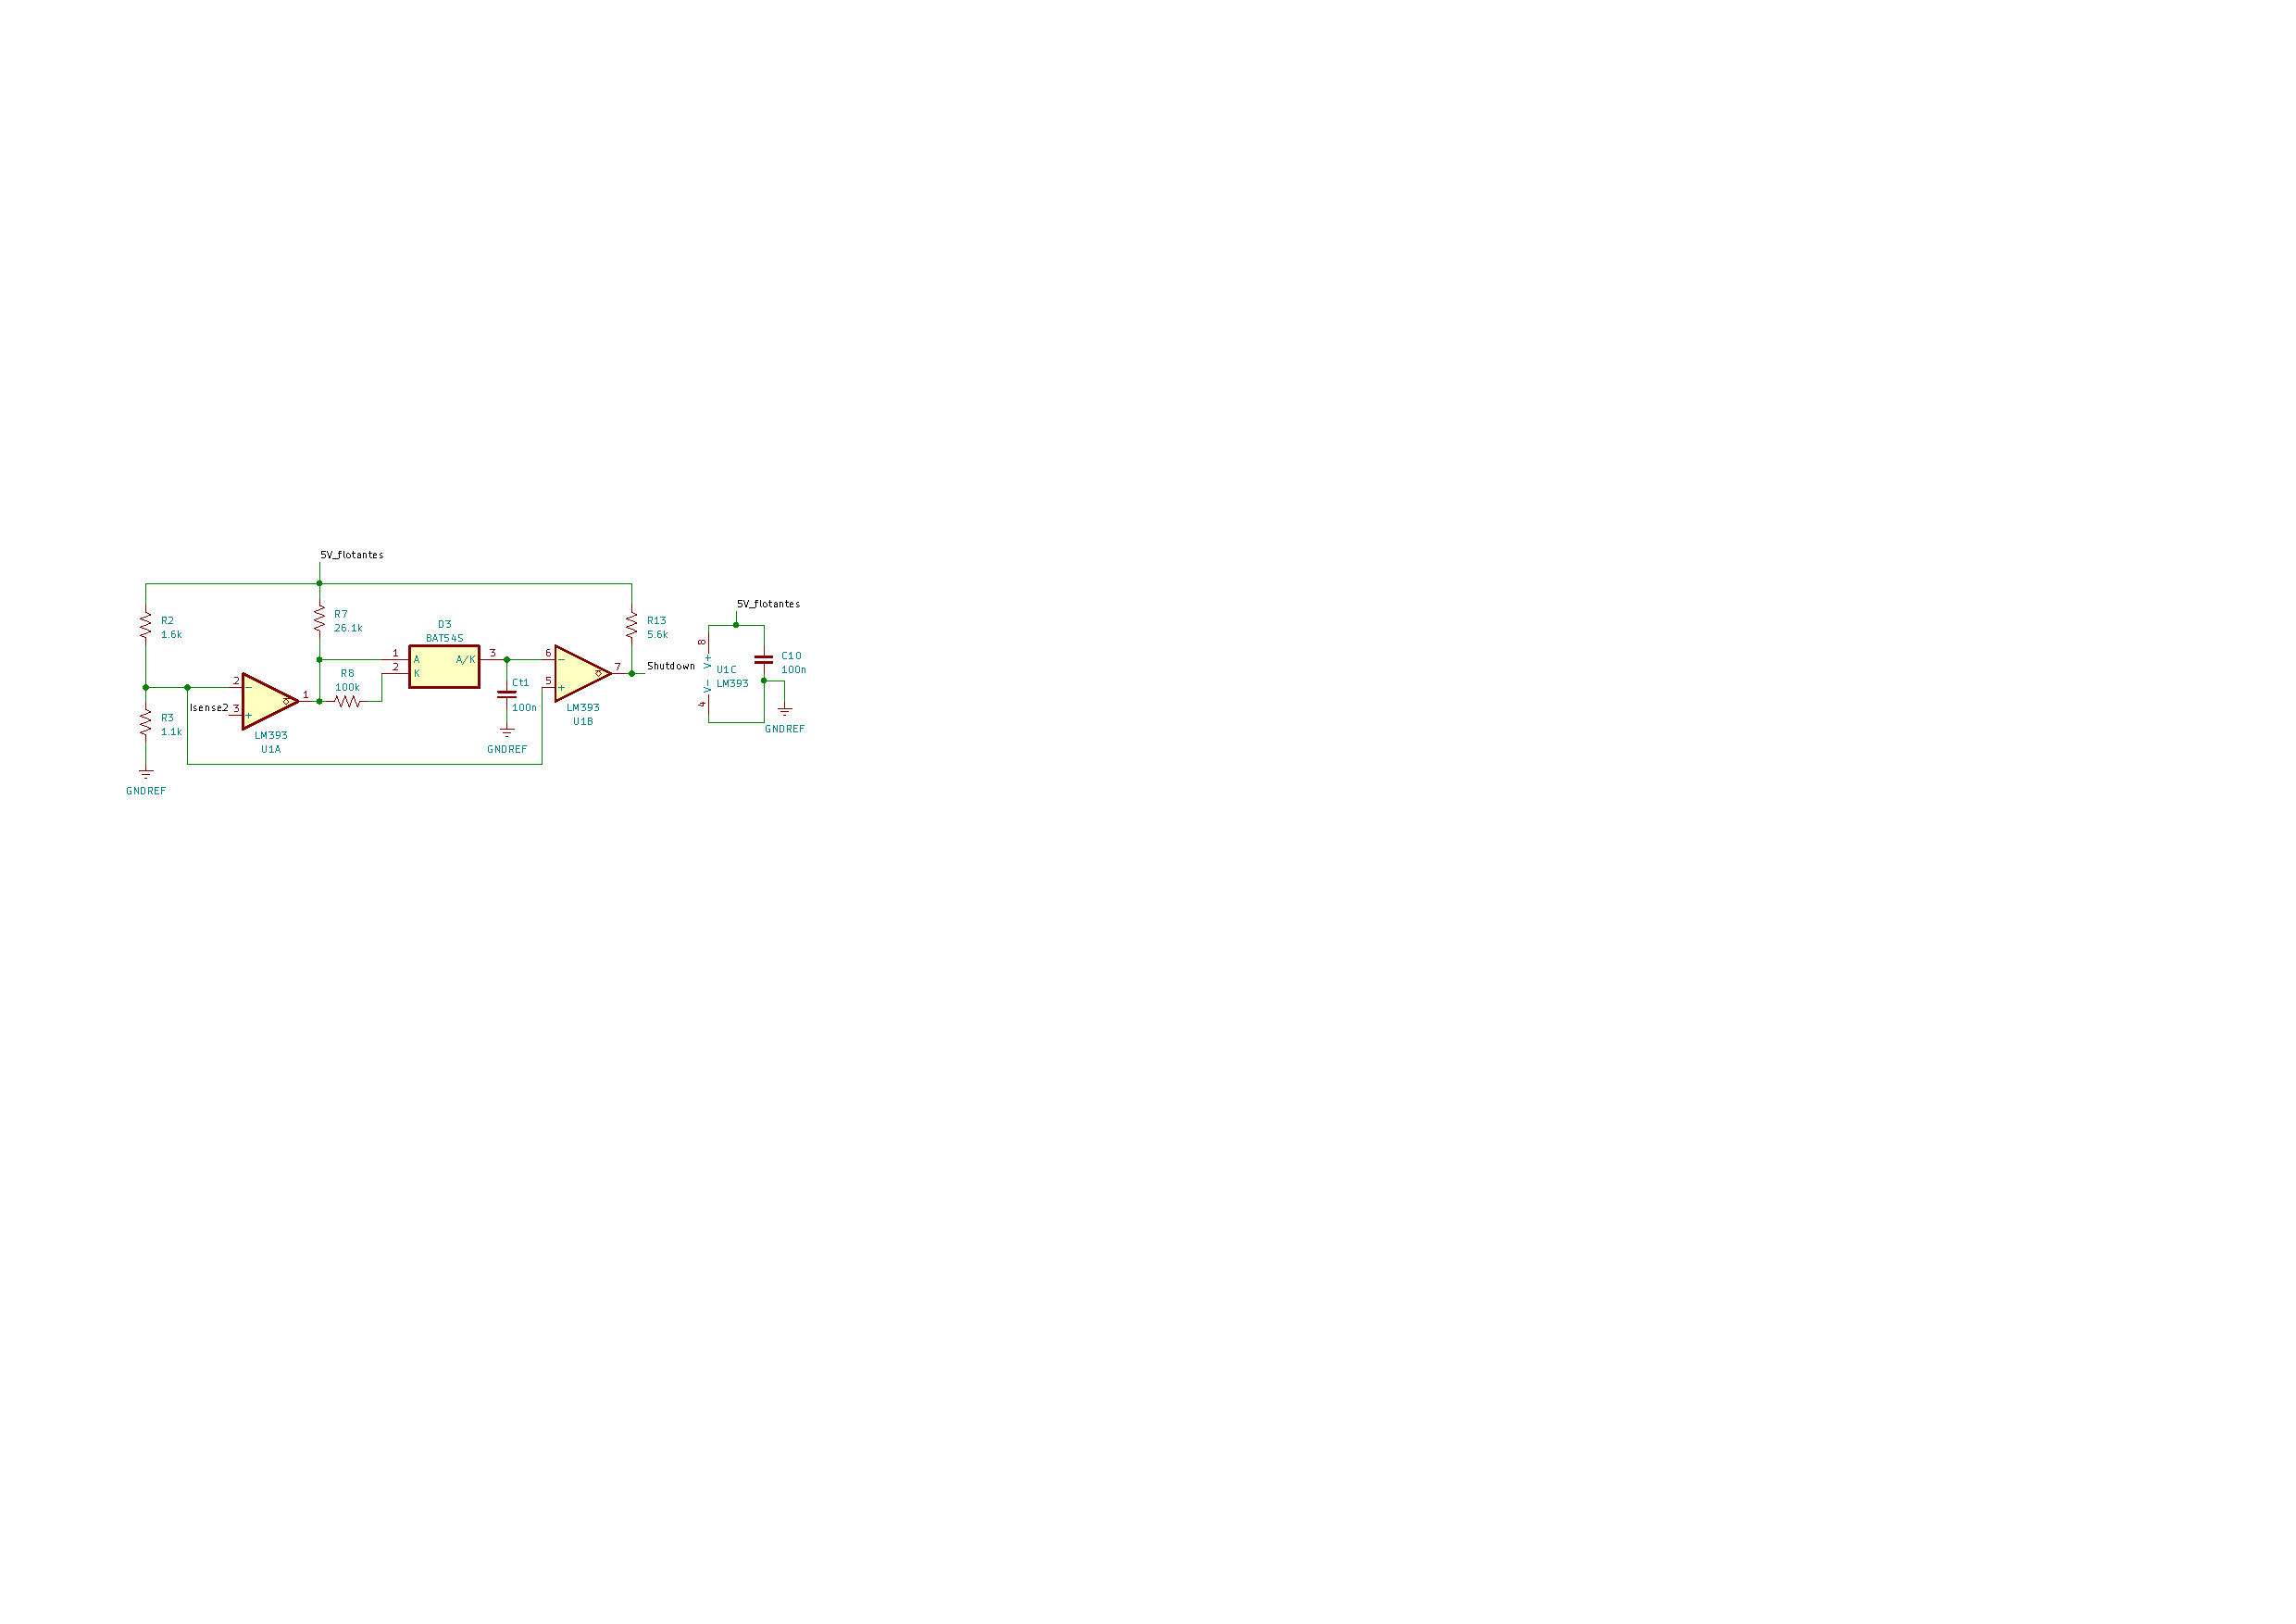
\includegraphics[width=0.92\textwidth]{TemporizadorKicadSch.pdf}\\
\small Temporizador asimétrico

\note{
El bloque de temporizador: dos comparadores LM393 en cascada, uno que detecta si se ha superado el umbral de 3,7 amperios y otro que vigila la carga del condensador de temporización a través de la red RC asimétrica, generando la señal de shutdown que, junto a la salida del biestable, entra en la puerta AND que finalmente habilita o deshabilita el driver del MOSFET.
}
\end{frame}

\begin{frame}
\transdissolve
\frametitle{Modelado en PSIM: potencia e histéresis}

\centering
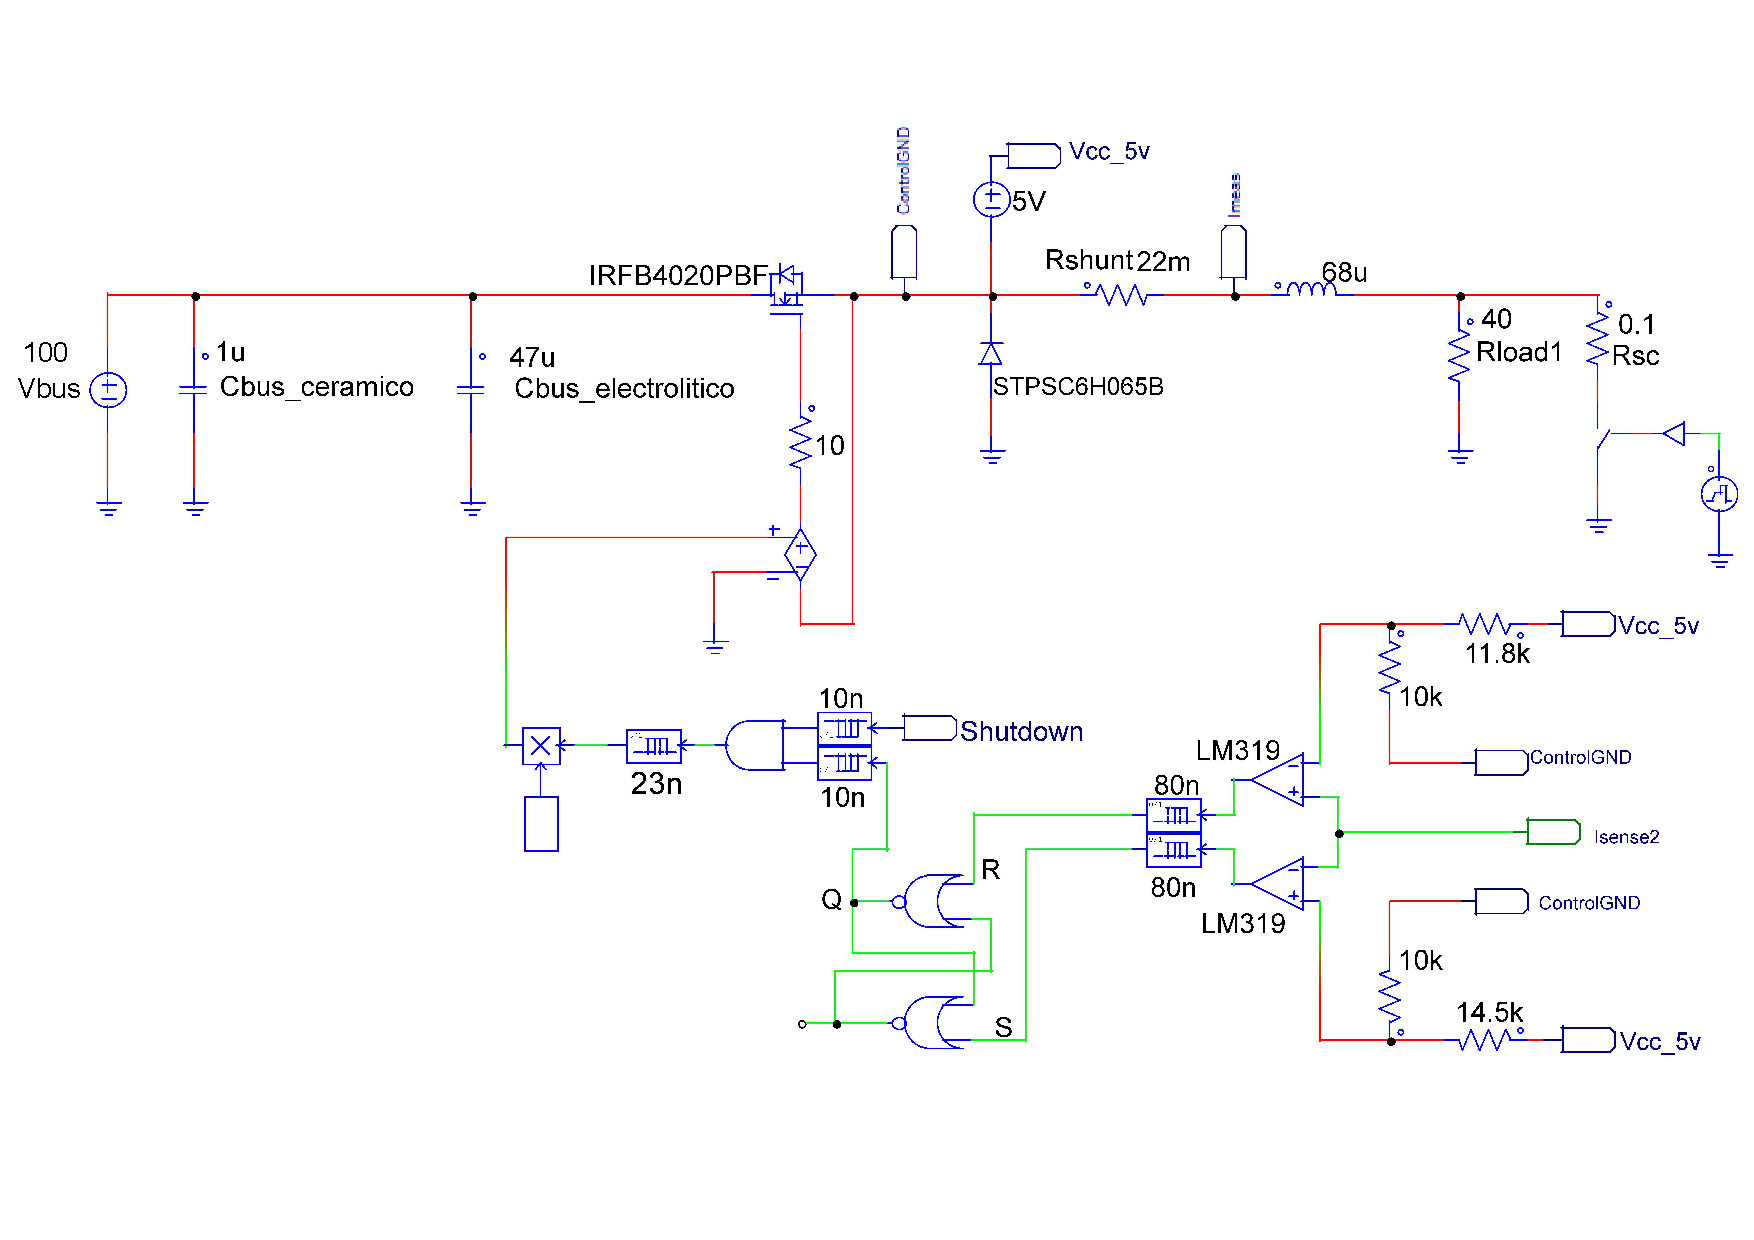
\includegraphics[width=0.78\textwidth]{Principal_psim.pdf}

\pause
\vspace{-0.15cm}
\small Retardos: comparador LM319 (80 ns) + puertas lógicas (10 ns) + driver (23 ns) $\approx$ \textbf{113 ns}.

\note{
Para que la simulación en PSIM sea representativa del hardware real no basta con un modelo ideal: se ha construido un modelo de comportamiento equivalente que incorpora los tiempos de propagación reales de los integrados elegidos. En concreto se han añadido bloques de retardo de 80 nanosegundos para el comparador LM319, 10 nanosegundos para las puertas lógicas y 23 nanosegundos para el driver UCC27511A, sumando unos 113 nanosegundos de retardo total en el lazo de histéresis. Esto es importante porque, por ese retardo entre la medida y el cambio de estado real del transistor, los límites de histéresis que se deben programar en el circuito tienen que ser ligeramente distintos a los teóricos para compensar el tiempo que tarda el sistema en reaccionar. También se simula el cortocircuito conectando una resistencia de 0,1 ohmios en paralelo con la carga nominal de 40 ohmios mediante un interruptor controlado por tensión.
}
\end{frame}

\begin{frame}
\transdissolve
\frametitle{Modelado en PSIM: acondicionamiento de señal}

\centering
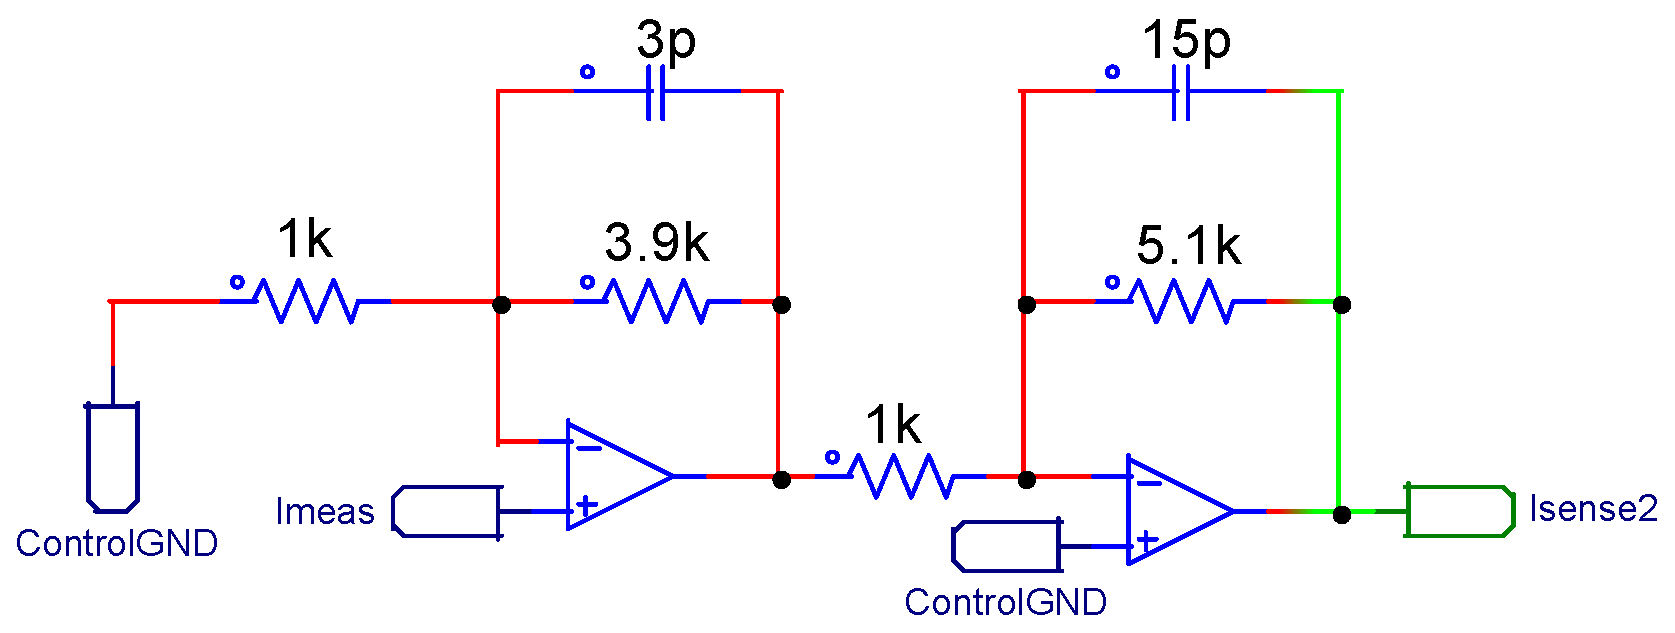
\includegraphics[width=0.95\textwidth]{Acondicionamiento_PSIM_recortado.pdf}\\
\small Acondicionamiento en cascada, idéntico al circuito real (parásitos del OPA2836)

\note{
La etapa de acondicionamiento analógico en PSIM replica de forma directa la topología en cascada diseñada en KiCad, garantizando una correspondencia exacta en ganancia y respuesta en frecuencia entre el circuito simulado y el hardware. Se emplean las características parásitas reales del OPA2836 para obtener un resultado lo más fiel posible a la realidad.
}
\end{frame}

\begin{frame}
\transdissolve
\frametitle{Modelado en PSIM: temporizador asimétrico}

\centering
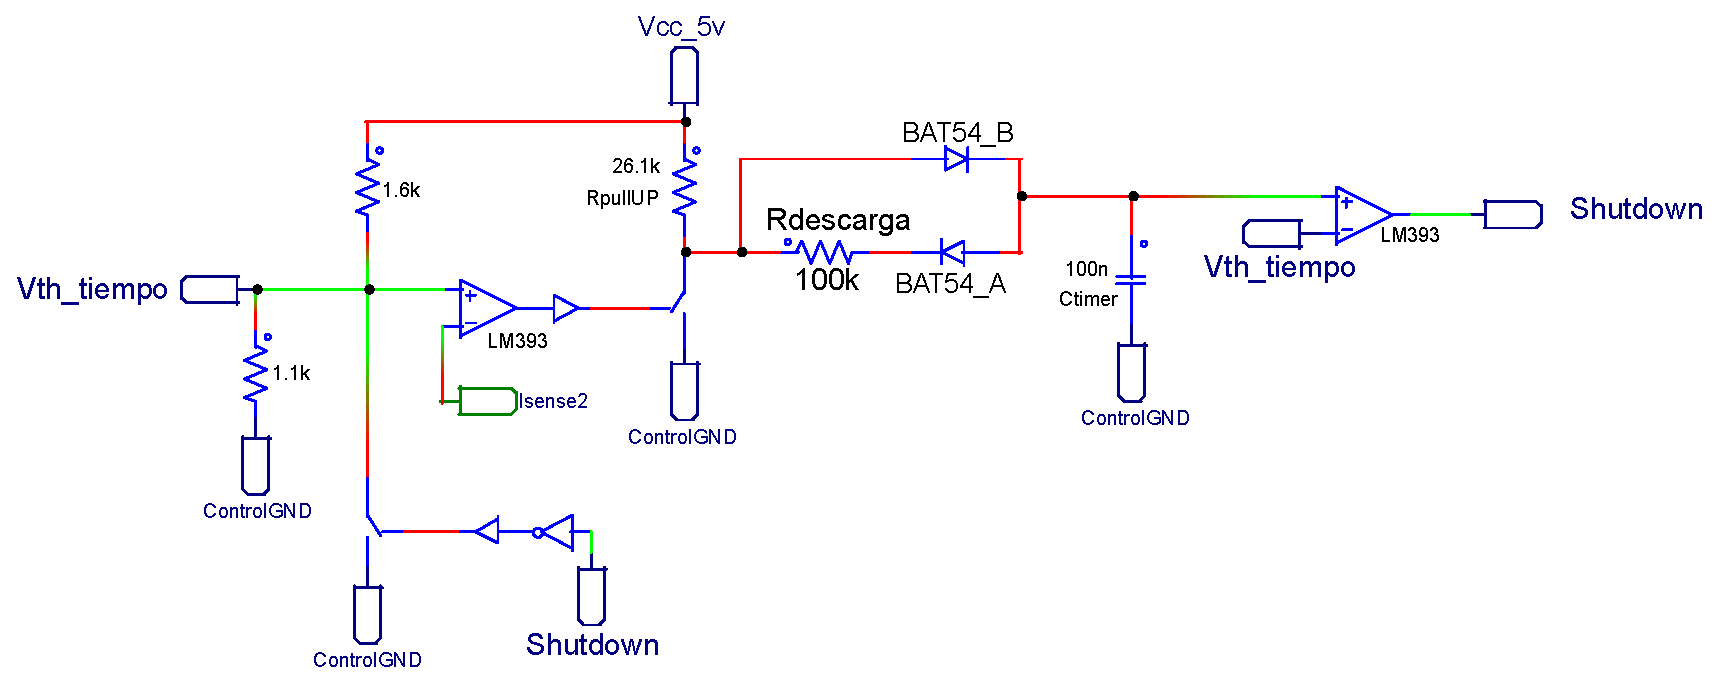
\includegraphics[width=0.95\textwidth]{Temporizador_PSIM_recortado.pdf}\\
\small Temporizador: colector abierto del LM393 emulado con interruptor controlado por tensión

\note{
El circuito de temporización se ha modelado según la arquitectura real, emulando el comportamiento de colector abierto del LM393 mediante un interruptor controlado por tensión. El mayor cambio respecto a la implementación real es el enclavamiento: se fuerza mediante un interruptor adicional que lleva la referencia a 0 voltios en el instante en que se activa la protección, imitando así el comportamiento del circuito físico una vez superado el trip-off time.
}
\end{frame}

\begin{frame}
\transdissolve
\frametitle{Resultado: respuesta ante fallo permanente}

\centering
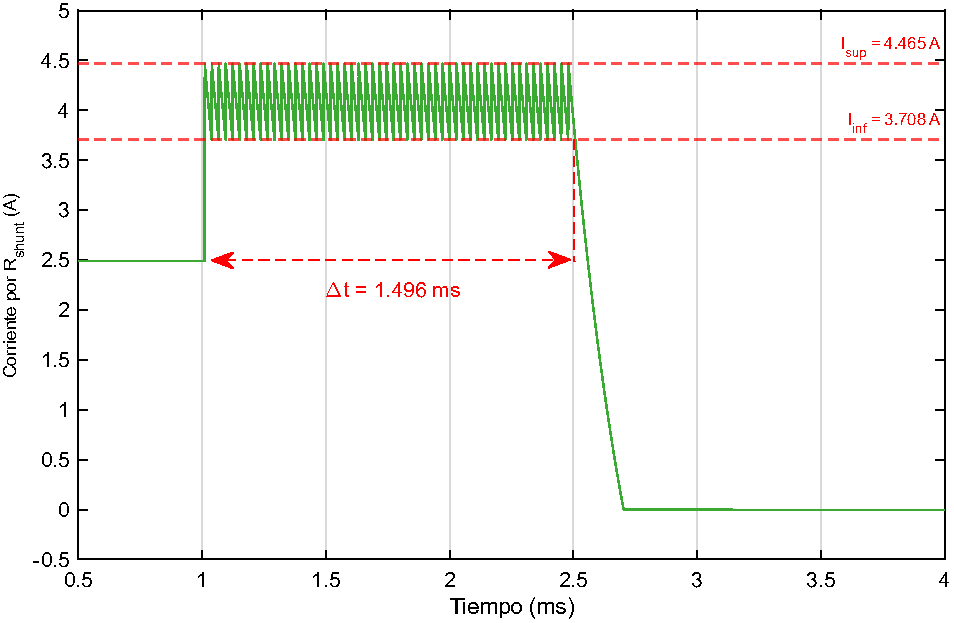
\includegraphics[width=0.64\textwidth]{Ishunt_fallo_permanente.pdf}

\vfill
\begin{itemize}
  \item Oscilación entre \textbf{3,708 A} y \textbf{4,465 A} (teórico: 3,7--4,5 A).
  \pause
  \item Enclavamiento a \textbf{1,496 ms} (objetivo: 1,5 ms).
\end{itemize}
\vspace{0.4cm}

\note{
Esta gráfica muestra la corriente por la resistencia de sensado tras introducir un cortocircuito en el instante 1 milisegundo. Se observa perfectamente el comportamiento esperado: la corriente oscila en conmutación entre 3,708 y 4,465 amperios, prácticamente idéntico a la banda teórica de 3,7 a 4,5 amperios, con la pequeña diferencia explicada por el retardo del lazo de control que vimos en la diapositiva anterior. Y tras 1,496 milisegundos de limitación, casi exactamente el objetivo de diseño de 1,5 milisegundos, el sistema se enclava y corta el paso de corriente. Este resultado valida tanto el dimensionado de la inductancia, que evita un sobrepico destructivo, como la precisión del temporizador.
}
\end{frame}

\begin{frame}
\transdissolve
\frametitle{Resultado: memoria térmica ante fallos sucesivos}

\centering
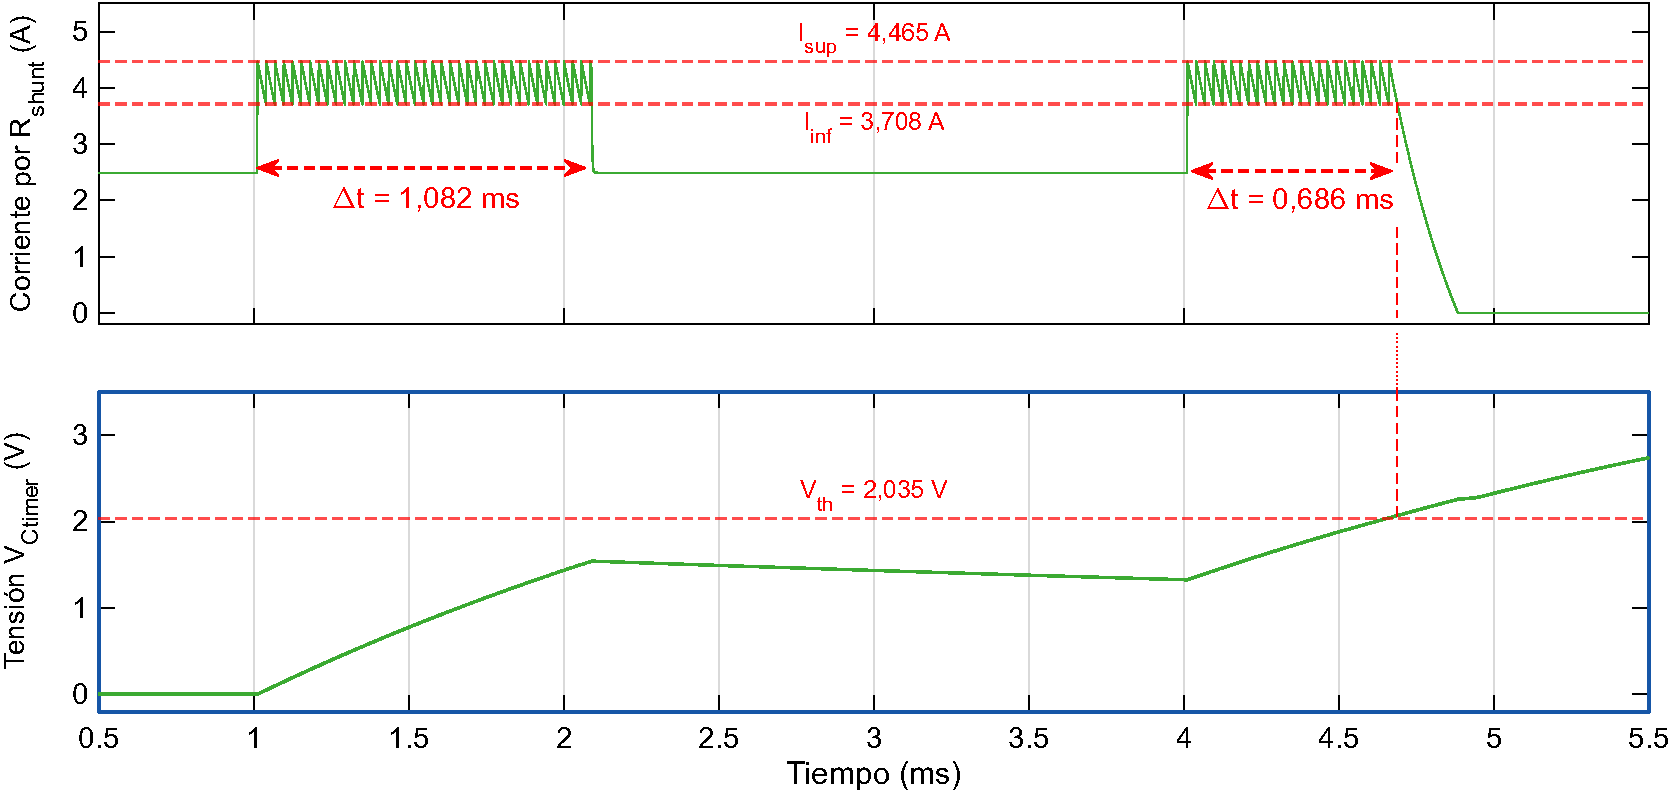
\includegraphics[width=0.8\textwidth]{IshuntvsVctimer1.pdf}

\vfill
\begin{itemize}
  \item Primer fallo: $V_\text{Ctimer}$ carga hasta $\approx 1{,}6$ V.
  \pause
  \item Sobrecorriente es transitoria: $V_\text{Ctimer}$ se descarga.
  \pause
  \item Segundo fallo a 4,7 ms (condensador no descargado): dispara en \textbf{0,686 ms}.
\end{itemize}
\vspace{0.4cm}

\note{
Aquí se somete al circuito a dos sobrecorrientes cercanas en el tiempo, simulando por ejemplo el arranque de un motor seguido de un cortocircuito real. Durante el primer fallo, de corta duración, el condensador del temporizador sube hasta aproximadamente 1,6 voltios y después se descarga lentamente por la red asimétrica. Cuando llega el segundo cortocircuito, a los 4,7 milisegundos, el condensador todavía conserva un voltaje residual de alrededor de 1,25 voltios porque no ha tenido tiempo de descargarse del todo, así que esta vez solo hace falta 0,686 milisegundos, en vez de 1,5, para alcanzar el umbral de disparo y enclavar el sistema. Esto confirma en simulación la memoria térmica del diseño: el sistema recuerda que el transistor no se ha enfriado y protege reduciendo el tiempo permitido de limitación.
}
\end{frame}

\begin{frame}
\transdissolve
\frametitle{Resultado: sincronización de la lógica de control}

\begin{columns}[c]
\column{0.53\textwidth}
\centering
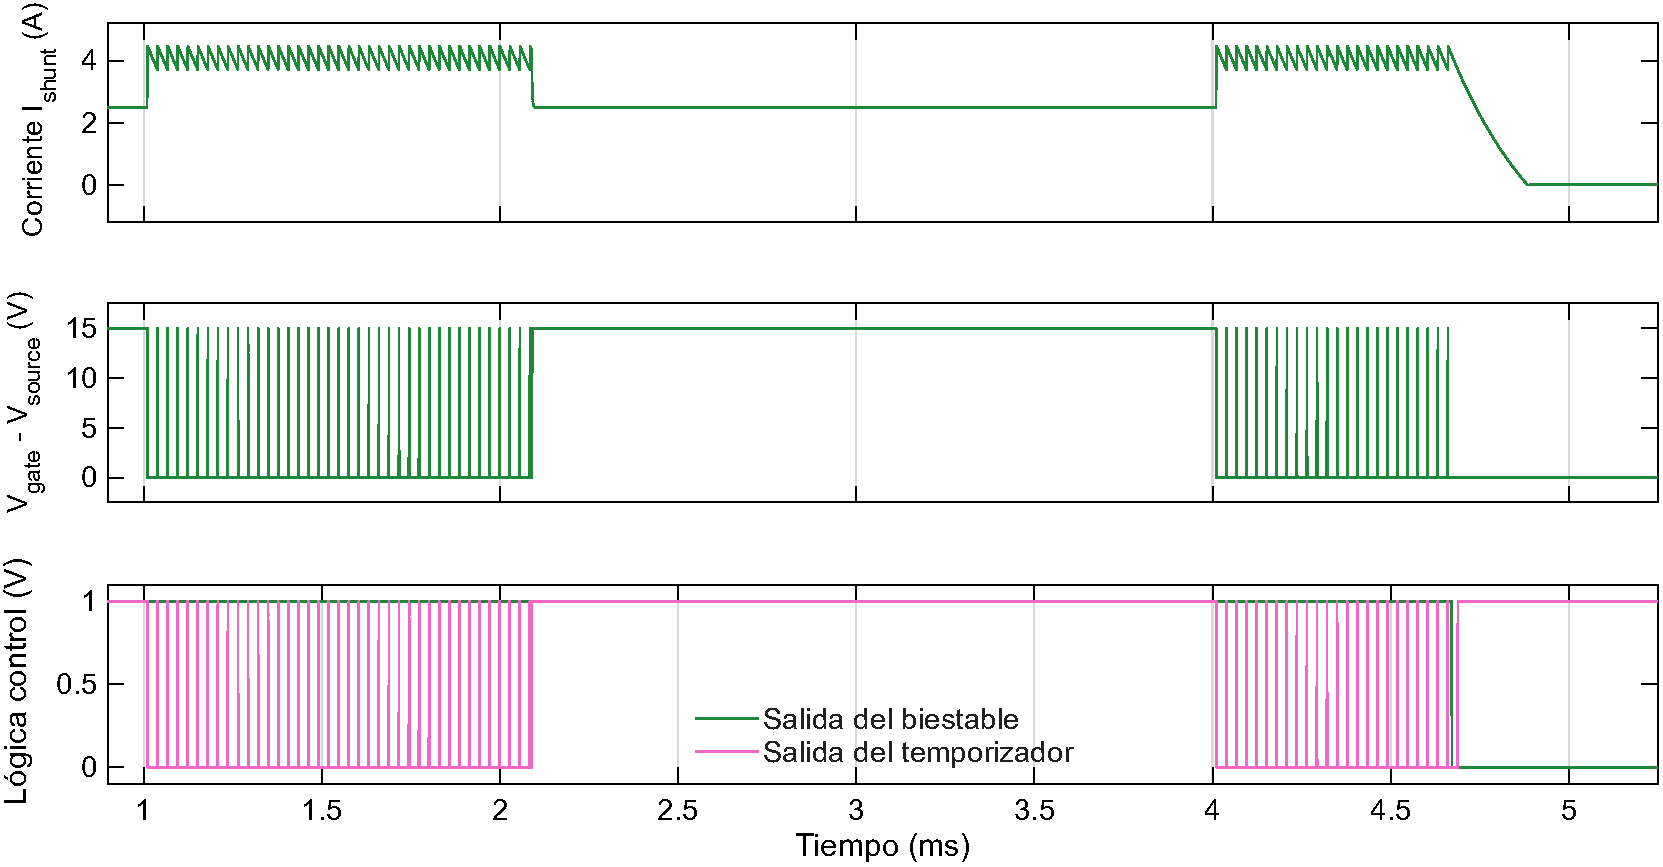
\includegraphics[width=\textwidth]{IvsVgsvsEntradasAND1.pdf}

\column{0.47\textwidth}
\onslide<2->{%
\centering
\resizebox{\textwidth}{!}{
\begin{tabular}{lcccc}
\toprule
\textbf{Fase} & \textbf{Hist.} & \textbf{Temp.} & \textbf{AND} & $\mathbf{V_\text{GS}}$ \\
\midrule
Nominal              & 1  & 1 & 1 & 15 V \\
Limitación (ON)      & 1  & 1 & 1 & 15 V \\
Limitación (OFF)     & 0  & 1 & 0 & 0 V \\
Enclavamiento        & -- & 0 & 0 & 0 V \\
\bottomrule
\end{tabular}
}}
\end{columns}

\vspace{0.25cm}
\onslide<3->{%
\centering
\small La \textbf{histéresis conmuta} (reversible); el \textbf{temporizador enclava} (hasta rearme).
}
\vspace{0.2cm}

\note{
Esta última gráfica de simulación es la comprobación de que los dos bloques de control, histéresis y temporizador, se coordinan como predice la máquina de estados que vimos antes. La tabla de la derecha es directamente esa máquina de estados traducida a niveles lógicos, y la clave es que la puerta AND solo deja pasar los 15 voltios a la puerta del MOSFET cuando ambas entradas están en uno. En nominal las dos están en uno y la puerta se mantiene fija a 15 voltios, sin conmutar. Durante la limitación el temporizador sigue en uno, pero la histéresis alterna entre uno y cero según la corriente sube o baja dentro de la banda, y por eso la tensión de puerta conmuta: es una fase reversible, si la corriente baja el sistema vuelve a nominal. Al superarse el tiempo de trip-off es el temporizador el que cae a cero, y como es una entrada de la AND, la tensión de puerta se queda a cero pase lo que pase con la histéresis; de ahí el guion en esa fila de la tabla. Esa es la diferencia esencial: la histéresis conmuta, el temporizador enclava.
}
\end{frame}

%==============================================================
\section{Validación Experimental}
%==============================================================

\begin{frame}
\transdissolve
\frametitle{Diseño de PCB: criterios de \textit{layout}}

\begin{columns}
\column{0.5\textwidth}
\begin{itemize}
  \item<1-> Lazo analógico y de potencia separados ($dv/dt$ y $di/dt$).
  \item<2-> \textit{Clearance} $>1{,}5$ mm entre planos de masa (IEC 60664-1).
  \item<3-> Pistas de potencia de 64 mil (IPC-2221C, $\Delta T=20\,^\circ$C).
  \item<4-> Desacoplo de alta frecuencia.
\end{itemize}
\column{0.5\textwidth}
\centering
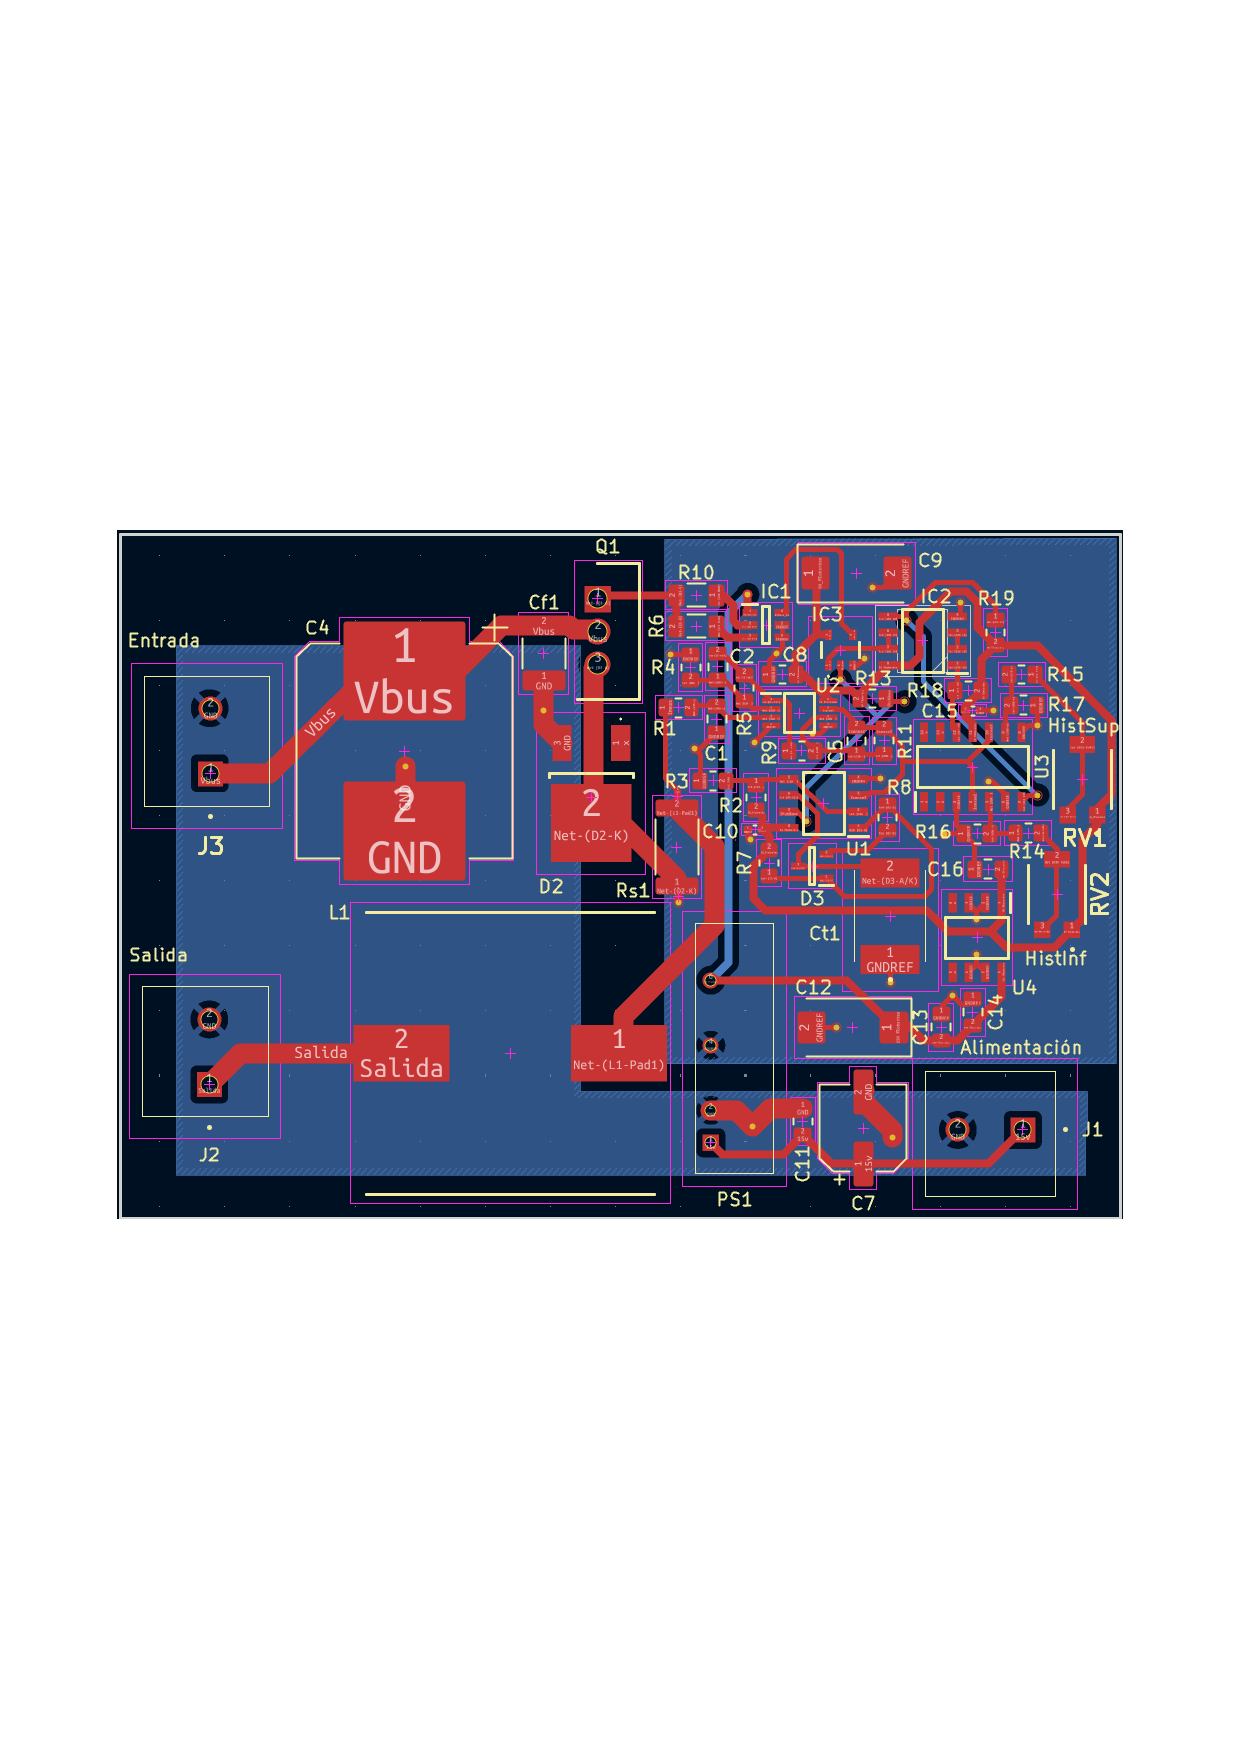
\includegraphics[width=\textwidth]{PCB_dibujoFallo.pdf}
\end{columns}

\note{
El diseño de la PCB en KiCad no es solo conectar componentes: a la frecuencia de conmutación de unos 600 kilohercios el layout condiciona directamente el ruido electromagnético. Se ha agrupado todo el lazo analógico, acondicionamiento, histéresis y temporización, en una zona compacta y separada de la etapa de alta corriente, para minimizar tanto el acoplo capacitivo por los campos eléctricos de conmutación como el acoplo magnético por los bucles de corriente. Entre los planos de masa, que pueden llegar a estar a 100 voltios de diferencia entre sí, se mantiene una distancia de al menos 1,5 milímetros, más que suficiente frente a la rigidez dieléctrica del aire y con margen frente a sobretensiones de conmutación. Las pistas de la etapa de potencia se han dimensionado a 64 mil siguiendo la norma IPC-2221C para no superar 20 grados de subida de temperatura, y los condensadores de desacoplo de alta frecuencia se han colocado lo más cerca posible de cada integrado y del drenador del MOSFET para minimizar la inductancia parásita de las trazas.
}
\end{frame}

\begin{frame}
\transdissolve
\frametitle{Incidencia de montaje: \textit{dead-bug wiring}}

\begin{columns}[c,onlytextwidth]
\column{0.44\textwidth}
\hspace*{-0.35cm}%
\begin{minipage}{\textwidth}
\centering
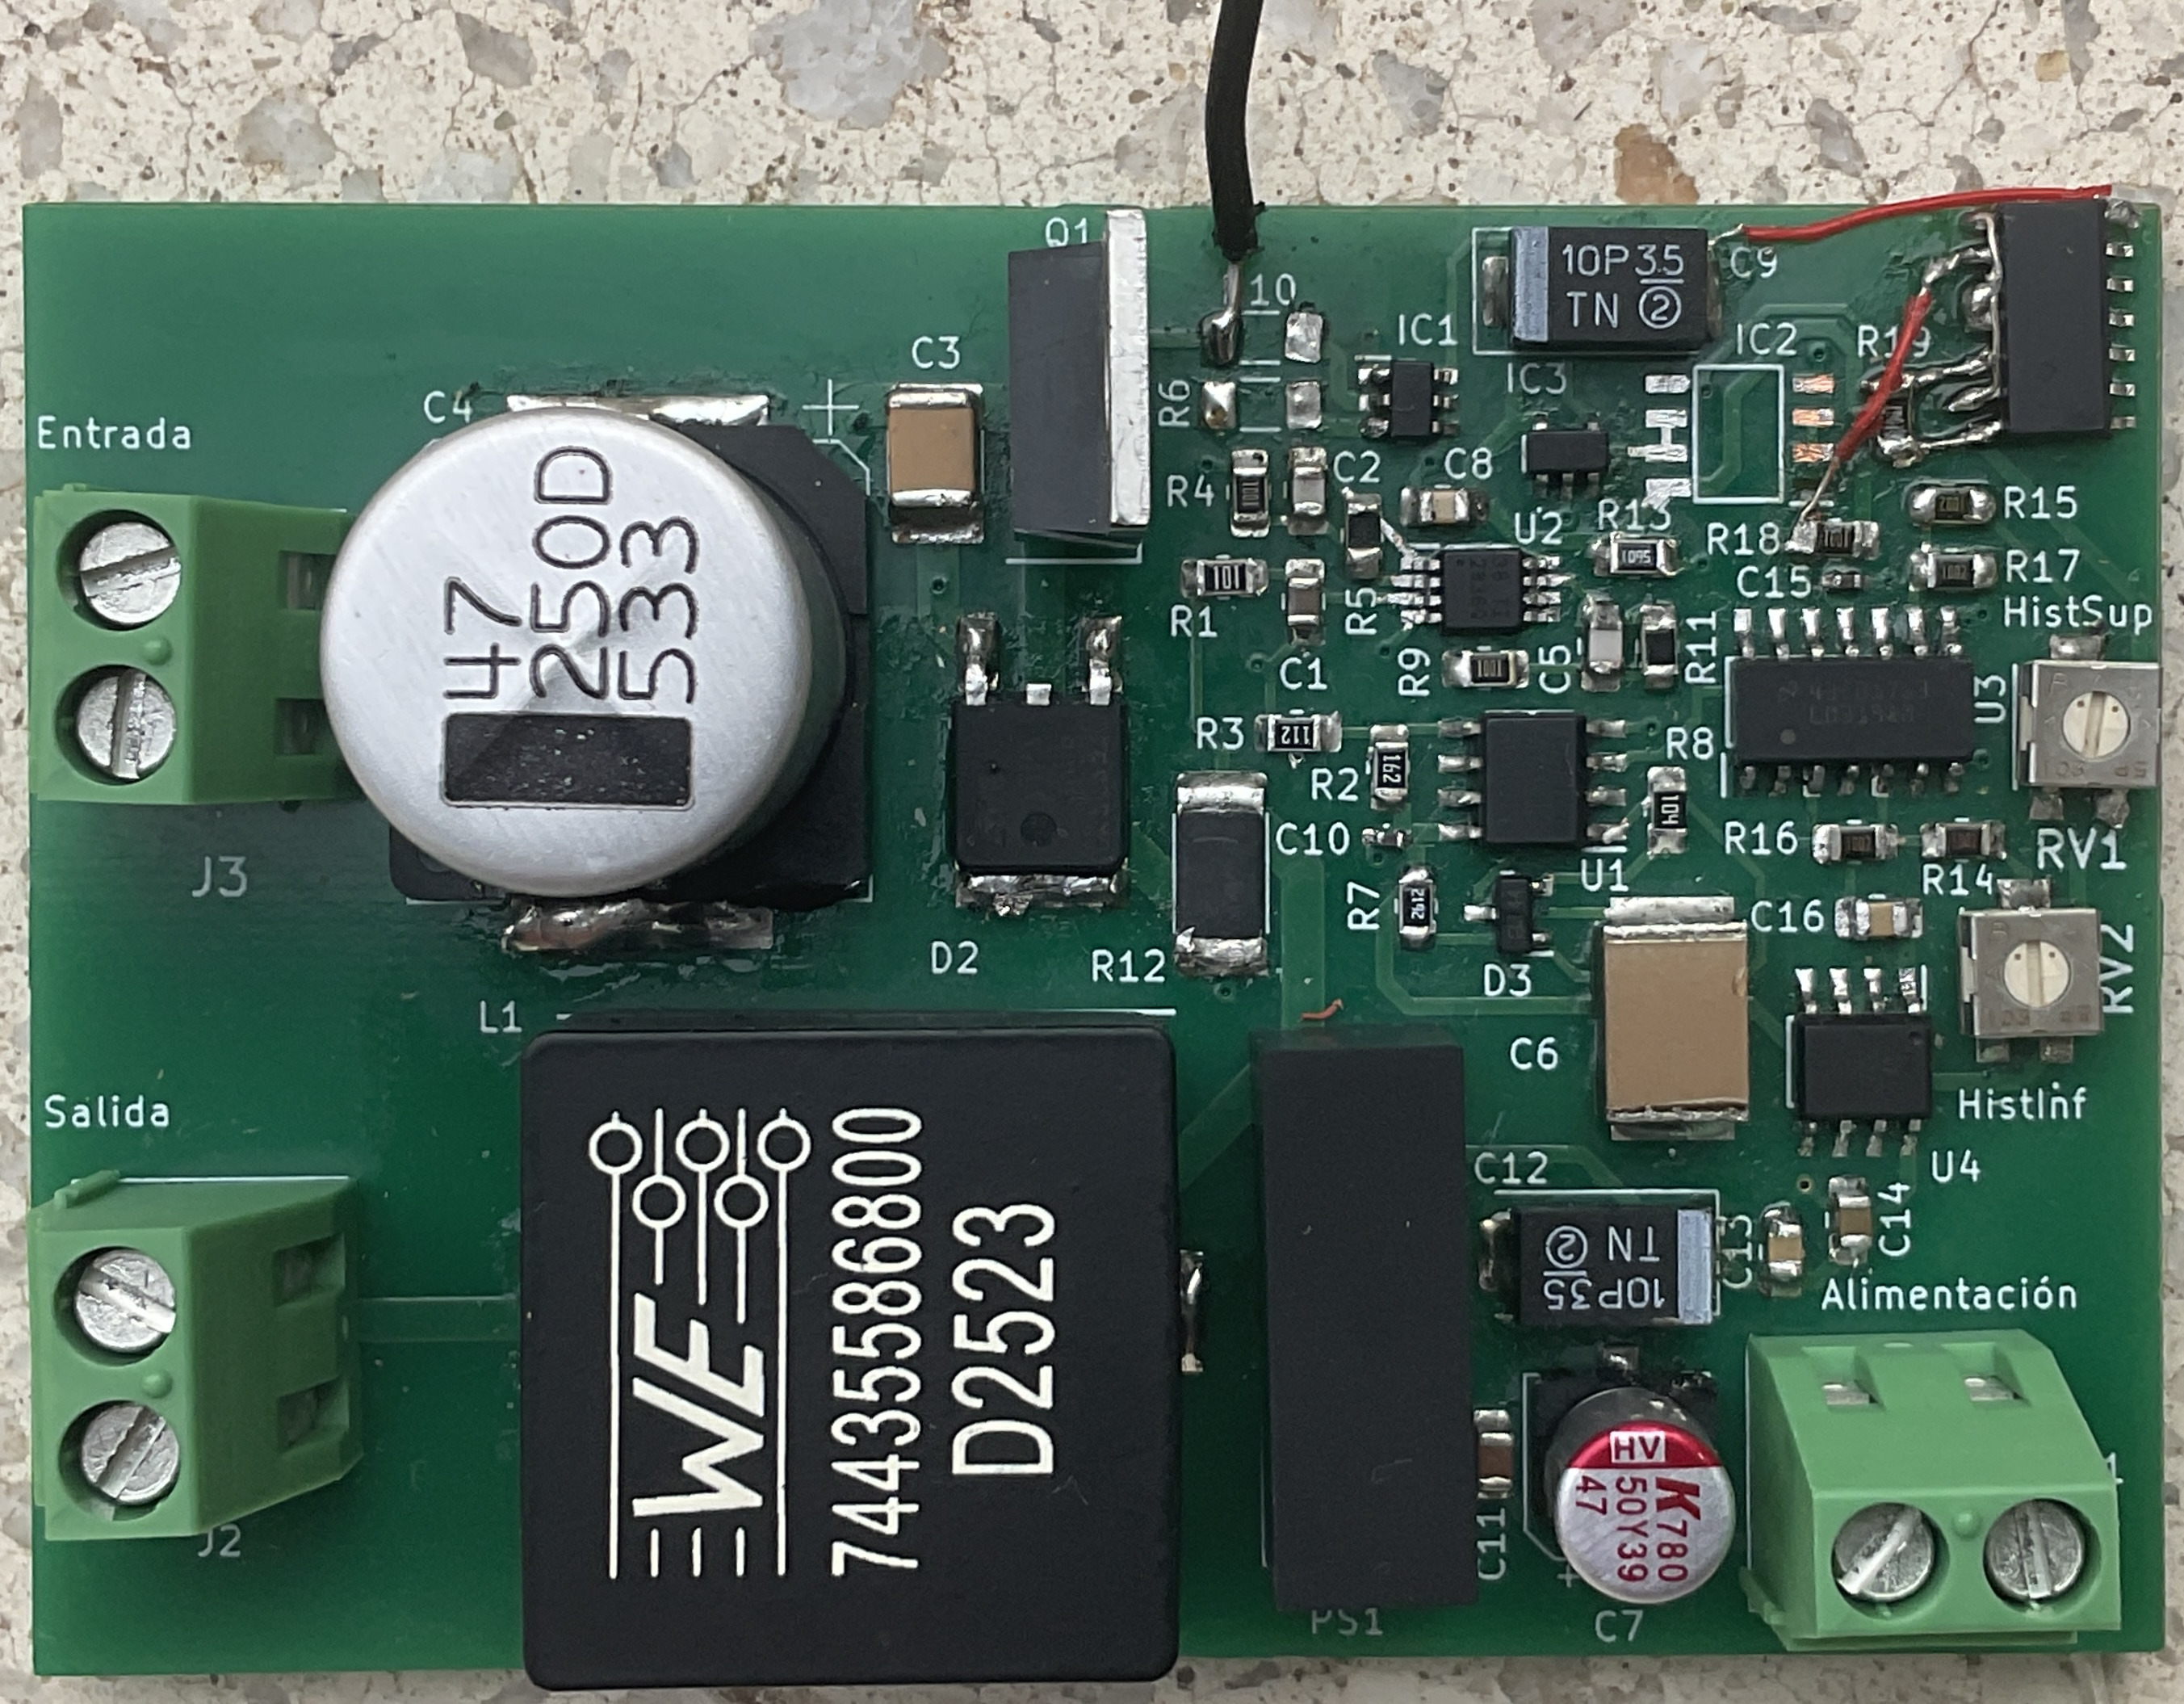
\includegraphics[height=0.58\textheight]{IMG_1484.jpg}\\
\footnotesize Montaje en araña sobre la PCB
\end{minipage}

\column{0.52\textwidth}
\centering
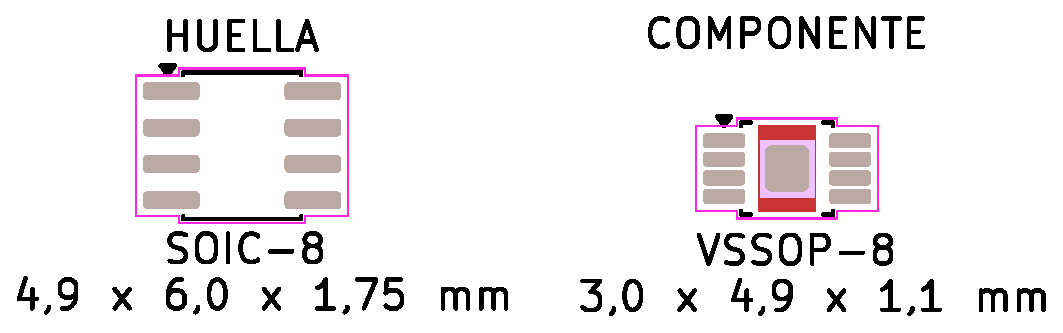
\includegraphics[width=\textwidth]{SOICvsVSSOP_recortado.pdf}\\
\footnotesize $1{,}27$ mm \textit{pitch} \quad vs \quad $0{,}5$ mm \textit{pitch}
\end{columns}

\vspace{0.2cm}
\pause
\centering
\textbf{Inductancia parásita} ($\approx 1$ nH/mm) $\Rightarrow V_\text{ruido}=L\,\dfrac{di}{dt}$ \\[0.6em]
\small Oscilaciones en comparador--biestable $\Rightarrow$ el \textit{driver} no excita la puerta de forma continua.
\vspace{0.2cm}

\note{
Durante el soldado manual de los componentes SMD se detectó que la huella descargada para la puerta NOR doble, encargada de formar el biestable RS, no coincidía con el encapsulado físico real: se había descargado una huella SOIC-8, mucho más grande, cuando el componente real era un VSSOP-8, con un paso entre pines demasiado pequeño para soldar cables directamente. En números, la huella SOIC-8 mide 4,9 por 3,91 milímetros con 1,27 milímetros entre pines, mientras que el VSSOP-8 real mide 2,3 por 2,0 milímetros con apenas 0,5 milímetros de paso, así que el integrado ni siquiera podía apoyarse dentro de la huella. La solución de emergencia fue un montaje en araña, dead-bug wiring, usando la misma función lógica en un integrado con mayor separación entre pines, el SN74LS02DR, fijado sobre la placa y conectado con cables finos hasta los pads originales; para acortar el recorrido, los cables se llevaron a componentes que ya compartían nodo con el pad. El problema es que estos cables aéreos tienen mucha más inductancia parásita que una pista de cobre, aproximadamente 1 nanohenrio por milímetro, y con las pendientes de corriente de la conmutación esa inductancia genera picos de tensión según la ecuación v igual a L por di/dt. Esos picos provocaron oscilaciones en los nodos que unen los comparadores con el biestable y, en consecuencia, la etapa de control perdió la capacidad de excitar de forma continua la puerta del MOSFET.
}
\end{frame}

\begin{frame}
\transdissolve
\frametitle{Ensayo experimental: tensión de entrada vs salida}

\centering
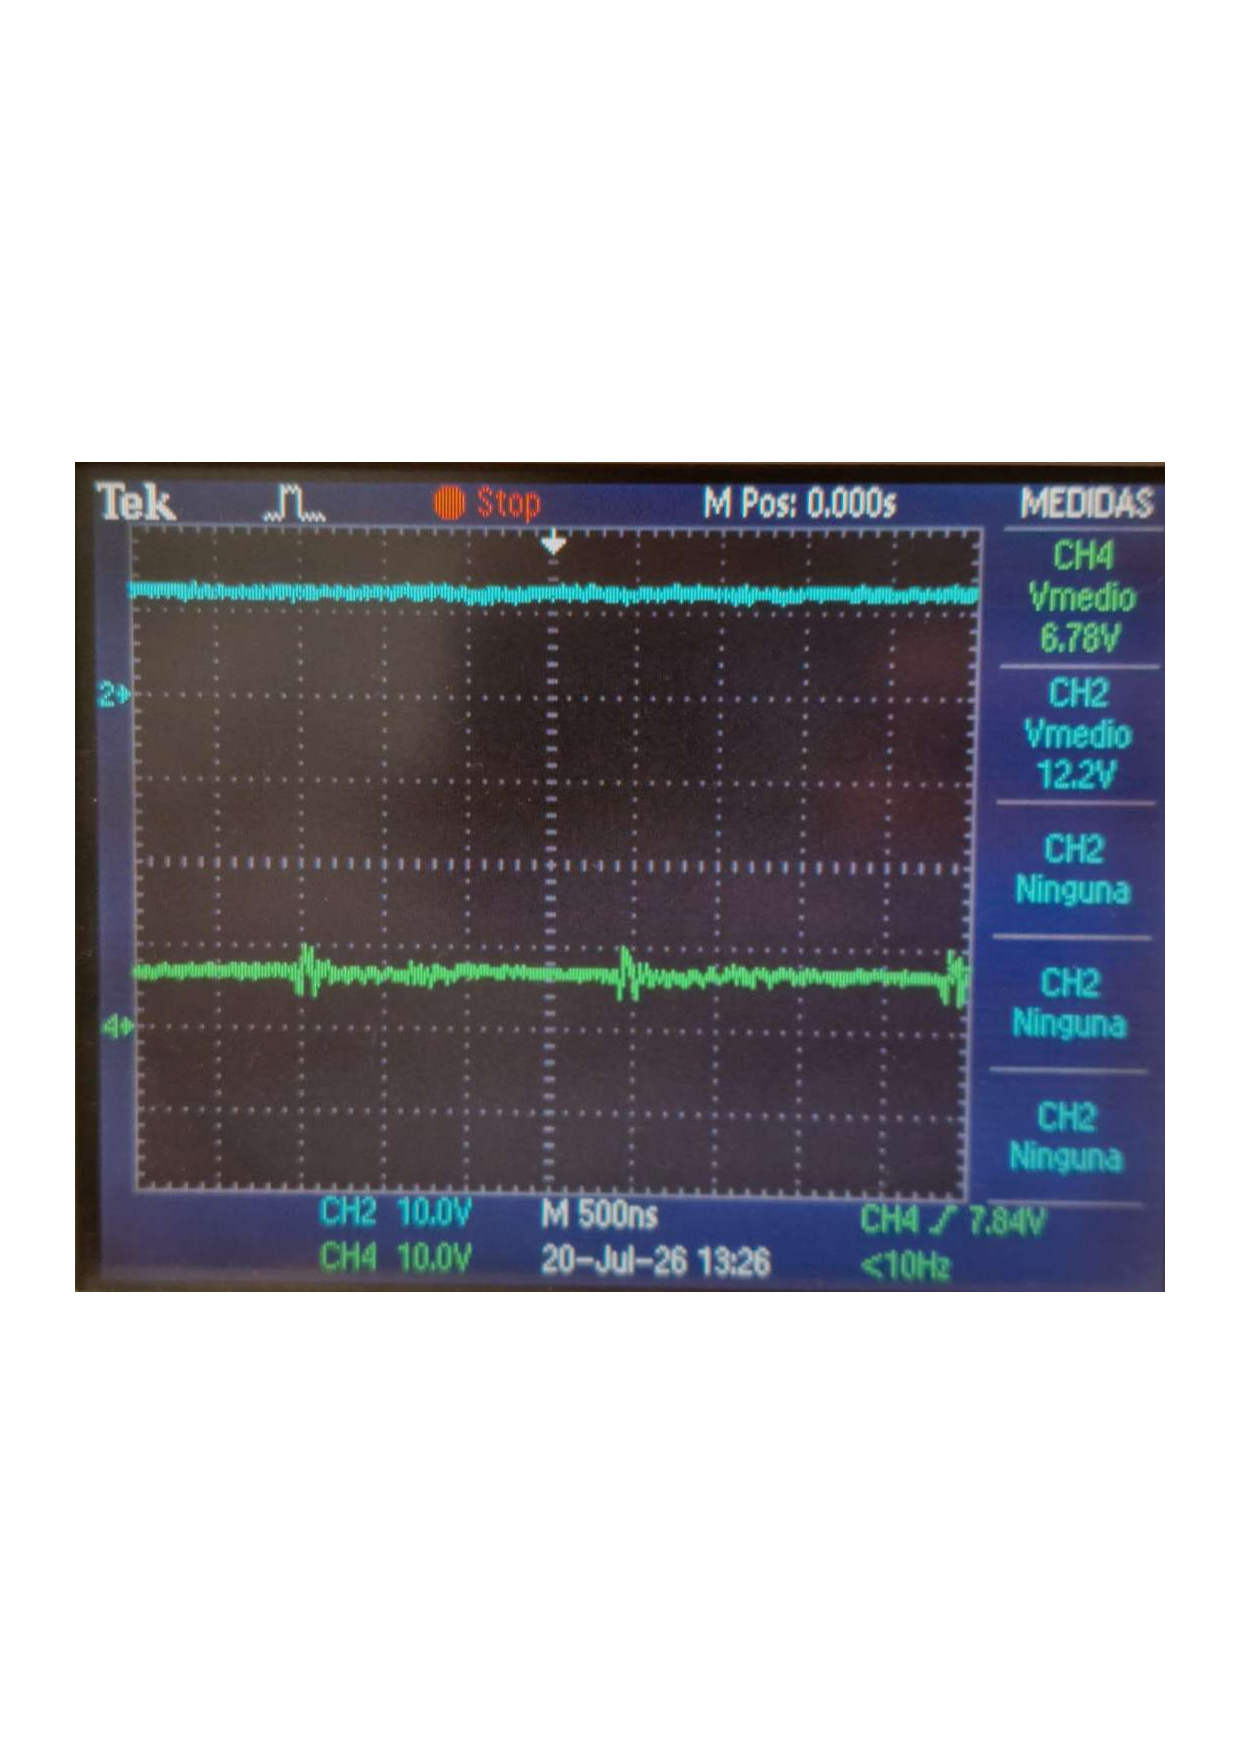
\includegraphics[width=0.62\textwidth]{20260720_132231_compressed.pdf}

\pause
\vspace{0.15cm}
\small $V_\text{in} = 12{,}2$ V (CH2) vs $V_\text{out} = 6{,}78$ V (CH4) $\Rightarrow$ $D\approx 0{,}65$ de PWM externo.

\note{
Esta captura del osciloscopio enfrenta la tensión de entrada al bus, en el canal 2, con la tensión de salida en la carga, en el canal 4. La salida es aproximadamente el 65 por ciento de la entrada, justo el ciclo de trabajo máximo que era capaz de dar el generador PWM externo. Además, como no hay condensador de salida y la señal solo está filtrada por la bobina, se aprecia el rizado de conmutación esperable superpuesto a la componente continua.
}
\end{frame}

\begin{frame}
\transdissolve
\frametitle{Ensayo experimental: filtrado inductivo y eficiencia}

\centering
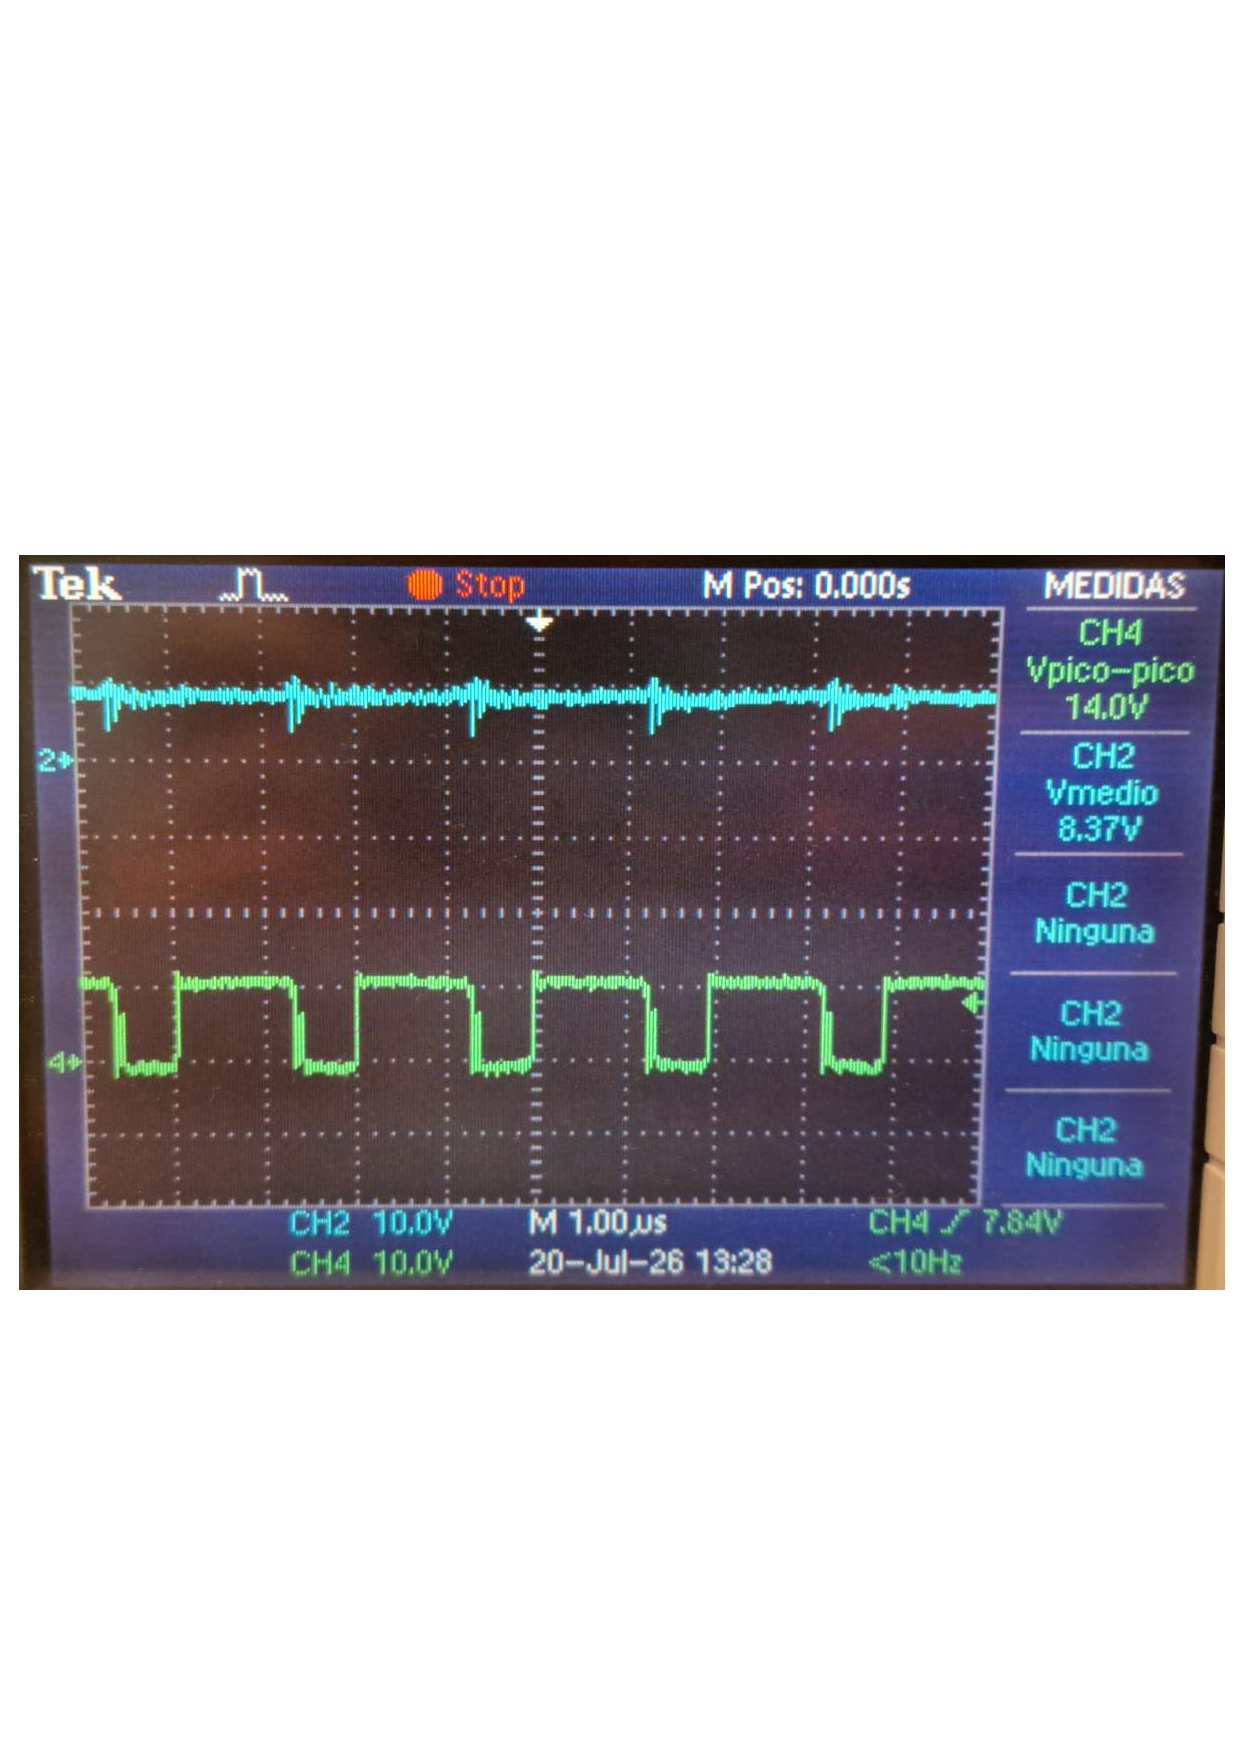
\includegraphics[width=0.55\textwidth]{20260720_132506_compressed.pdf}
\\ \small Tensión pre-bobina (conmutada) vs post-bobina (constante).

\pause
\vfill
\begin{itemize}
  \item Excitación con PWM externo ($f_\text{sw}\approx508$ kHz, $D\approx0{,}65$).
  \pause
  \item Bobina (68 $\mu$H): conmutación $\rightarrow$ salida continua y estable.
  \pause
  \item $\eta_\text{medida}~=~$\textbf{89,2 \%} a 12,2 V vs $\eta_\text{teórica}~=~$\textbf{96,5 \%} a 100 V
\end{itemize}

\note{
Como el fallo de montaje impidió que la etapa de control disparase el driver de forma continua, se decidió aislar y validar únicamente la etapa de potencia: se desoldaron las resistencias de entrada a la puerta y se inyectó un PWM externo directamente en la fuente del transistor, a una frecuencia de unos 508 kilohercios, muy cercana a los 615 kilohercios teóricos, aunque limitada a un ciclo de trabajo máximo de 0,65 por las limitaciones del generador externo. La imagen del osciloscopio muestra la tensión antes de la bobina, una onda cuadrada con sobreoscilaciones, frente a la tensión después de la bobina, una señal prácticamente continua y estable, demostrando que el filtrado inductivo funciona correctamente incluso sin condensador de salida. En estas condiciones, a un bus reducido de 12,2 voltios por seguridad de laboratorio, se midió una eficiencia del 89,2 por ciento, inferior al 96,5 por ciento teórico a tensión nominal de 100 voltios, porque a menor tensión las caídas parásitas del diodo y las resistencias pesan proporcionalmente mucho más.
}
\end{frame}

\begin{frame}
\transdissolve
\frametitle{Limitaciones del ensayo}

\begin{columns}[T]
\column{0.5\textwidth}
\centering
\textbf{\textcolor{green!55!black}{Validado en laboratorio}}
\begin{itemize}
  \item[\textcolor{green!55!black}{\checkmark}] Etapa de potencia en \textit{high-side}
  \pause
  \item[\textcolor{green!55!black}{\checkmark}] Filtrado inductivo (68 $\mu$H)
  \pause
  \item[\textcolor{green!55!black}{\checkmark}] Eficiencia medida (89,2 \%)
\end{itemize}

\column{0.5\textwidth}
\pause
\centering
\textbf{\textcolor{red!70!black}{Pendiente de validar}}
\begin{itemize}
  \item[\textcolor{red!70!black}{$\times$}] Conmutación completa del lazo de histéresis
  \pause
  \item[\textcolor{red!70!black}{$\times$}] Enclavamiento real
  \pause
  \item[\textcolor{red!70!black}{$\times$}] Memoria térmica en \textit{hardware}
\end{itemize}
\end{columns}

\pause
\vspace{0.3cm}
\centering
\small Posible causa: montaje en araña $\Rightarrow$ inestabilidad del biestable + potenciómetros sin rango para cargas de laboratorio seguras.

\note{
No todo pudo validarse en el laboratorio, pero conviene separar claramente lo que sí se demostró de lo que queda pendiente. Se validó experimentalmente el funcionamiento de la etapa de potencia en configuración high-side, la capacidad de filtrado inductivo de la bobina de 68 microhenrios, y se midió una eficiencia del 89,2 por ciento en las condiciones de ensayo. Quedó pendiente, en cambio, comprobar la conmutación completa del lazo de histéresis, el enclavamiento real ante un fallo, y la memoria térmica sobre el hardware físico. La causa común de estas tres limitaciones es la misma: el montaje en araña introdujo inestabilidad en el biestable que impidió excitar el driver de forma continua, y además los potenciómetros de ajuste de histéresis no tienen rango suficiente para bajar la corriente de limitación a un valor medible con las cargas de laboratorio disponibles de forma segura. Ambas cosas quedan como primeras tareas de la siguiente iteración del prototipo.
}
\end{frame}

%==============================================================
\section{Escalado y Conclusiones}
%==============================================================

\begin{frame}
\transdissolve
\frametitle{Metodología de escalado}

\begin{table}
\centering
\renewcommand{\arraystretch}{2.1}
\resizebox{\textwidth}{!}{
\begin{tabular}{clp{11.5cm}}
\toprule
\textbf{\#} & \textbf{Parámetro} & \textbf{Qué hay que modificar} \\
\midrule
1 & $V_\text{bus}$, $I_\text{nom}$ & MOSFET, diodo y bobina ($I_\text{sat}$). $P_\text{shunt}<0{,}5$ W \\
2 & $I_\text{lim}$ & $V_\text{TimON}=I_\text{lim}\cdot R_\text{shunt}\cdot G \ \rightarrow$ Divisor de entrada al temporizador \\
3 & $t_\text{trip}$ & Con $C_\text{timer}$ fijado, ajustar $\tau$ mediante $R_\text{carga}$  \\
4 & $\Delta i$ & $R_\text{var,1}$ y $R_\text{var,2}$: $V_\text{sup/inf}=I_\text{hys,sup/inf}\cdot R_\text{shunt}\cdot G$ \\
\bottomrule
\end{tabular}
}
\end{table}

\pause
\vspace{0.2cm}
\centering
\small $\Delta i$ fija $f_\text{sw}$: banda estrecha $\Rightarrow \uparrow P_\text{sw}$ y disparos falsos por ruido.

\note{
Uno de los objetivos del trabajo era que el diseño no fuera válido solo para estas especificaciones concretas, sino que se pudiera adaptar fácilmente a otros casos de uso. La tabla está ordenada como hay que hacerlo, porque los pasos dependen unos de otros. Primero, si cambia la tensión de bus o la corriente nominal, hay que revisar la etapa de potencia: que el MOSFET aguante la tensión drenador-surtidor y no supere los 125 grados de unión, que el diodo sea adecuado, que la bobina no sature con el pico de corriente, y que la resistencia de sensado siga disipando por debajo de los 0,5 vatios de su encapsulado. Segundo, la corriente de limitación: no se toca ningún componente de potencia, lo que se cambia es la tensión de referencia del temporizador, que es simplemente la corriente nueva por la resistencia de sensado por la ganancia de 25; esa tensión se fija con la relación entre las dos resistencias del divisor alimentado a 5 voltios. Tercero, el tiempo de trip-off: se deja el condensador en los 100 nanofaradios, que es un valor comercial estable, y se despeja la resistencia de carga de la exponencial; hay que hacerlo después de la corriente de limitación porque la tensión de referencia aparece en esa fórmula. Y cuarto, la banda de histéresis, que se ajusta en los dos potenciómetros de los comparadores, calculando la tensión de cada umbral igual que antes: corriente por resistencia de sensado por ganancia. Un aviso importante en este último punto: la anchura de la banda es lo que fija la frecuencia de conmutación, así que una ventana demasiado estrecha dispara las pérdidas dinámicas del MOSFET y hace el sistema vulnerable a disparos falsos por ruido. La idea de fondo es que la topología y los bloques no cambian: solo se recalculan los valores de un número muy reducido de componentes.
}
\end{frame}

\begin{frame}
\transdissolve
\frametitle{Conclusiones y logros alcanzados}

\begin{enumerate}
  \item \textbf{Demostración teórica y simulada:} topología N-MOS conmutada
   frente a los LCL lineales en alta tensión (100 V).
  \pause
  \item \textbf{Diseño validado en simulación:} limitación (3,708--4,465 A) y temporización (1,496 ms vs. 1,5 ms objetivo) precisas.
  \pause
  \item \textbf{Etapa de potencia funcional en hardware:} conmutación $\uparrow f$  en \textit{high-side} con filtrado inductivo ($\eta~=~89,2 \% $ a baja tensión).
\end{enumerate}

\note{
En resumen, este trabajo demuestra, primero a nivel teórico y después en simulación con parásitos reales, que la topología N-MOS en conmutación resuelve el problema térmico que limita a los LCL lineales tradicionales cuando se sube a buses de alta tensión como los 100 voltios. El diseño se ha validado en PSIM con una precisión muy alta tanto en los límites de histéresis, 3,708 a 4,465 amperios frente a los 3,7 a 4,5 teóricos, como en el temporizador, 1,496 milisegundos frente al 1,5 objetivo. Y, aunque el lazo de control completo no pudo validarse en el laboratorio por el problema de montaje, sí se ha demostrado de forma experimental que la etapa de potencia funciona correctamente en configuración high-side a alta frecuencia de conmutación, con un filtrado inductivo eficaz y una eficiencia medida del 89,2 por ciento incluso en las condiciones desfavorables de baja tensión del ensayo.
}
\end{frame}

\begin{frame}
\transdissolve
\frametitle{Líneas futuras}

\centering
\resizebox{0.92\textwidth}{!}{
\begin{tikzpicture}[every node/.style={font=\small, align=center}]
  \path[use as bounding box] (-2.3,-1.1) rectangle (13.1,1.1);
  \node[draw, rectangle, rounded corners, fill=red!8, minimum width=4.3cm, minimum height=1.8cm] (paso1) at (0,0) {\textbf{1. Corrección PCB}\\[2pt] Huella \\ y lazo de control};
  \node<3->[draw, rectangle, rounded corners, fill=yellow!12, minimum width=4.3cm, minimum height=1.8cm] (paso2) at (5.4,0) {\textbf{2. Validar a 100 V}\\[2pt] Histéresis y enclavamiento\\ con cargas de potencia};
  \node<5->[draw, rectangle, rounded corners, fill=green!10, minimum width=4.3cm, minimum height=1.8cm] (paso3) at (10.8,0) {\textbf{3. Calificación espacial}\\[2pt] Componentes \textit{rad-hard}\\ y fijación mecánica};
  \draw<3->[-latex, line width=1.4pt] (paso1) -- (paso2);
  \draw<5->[-latex, line width=1.4pt] (paso2) -- (paso3);
\end{tikzpicture}
}

\vspace{0.35cm}
\begin{columns}[t]
\column{0.32\textwidth}
\onslide<2->{\footnotesize
\begin{itemize}
  \item Potenciómetros de mayor rango.
  \item \textit{Clearance} y anchos de vía según normativa.
\end{itemize}}

\column{0.32\textwidth}
\onslide<4->{\footnotesize
\begin{itemize}
  \item $t_\text{trip}$ real frente a los $1{,}5$ ms.
  \item Memoria térmica ante fallos sucesivos.
\end{itemize}}

\column{0.32\textwidth}
\onslide<6->{\footnotesize
\begin{itemize}
  \item SiC/GaN: misma topología, $\uparrow f_\text{sw}$.
  \item Estudios mecánicos: vibraciones del lanzamiento.
\end{itemize}}
\end{columns}

\note{
De cara a las siguientes iteraciones del prototipo, hay tres líneas de trabajo claras y secuenciales. La primera y más urgente es corregir la huella de la PCB al encapsulado VSSOP-8 correcto y rediseñar el lazo de control para reducir aún más el acoplo magnético, eliminando así el montaje en araña y su inductancia parásita; en esa misma revisión conviene montar potenciómetros con más rango, porque los actuales no permiten bajar los umbrales de histéresis a corrientes que se puedan ensayar con seguridad en el laboratorio, y revisar ya los clearances y los anchos de vía para que cumplan lo que exigen las autoridades certificadoras. La segunda es completar la validación experimental que quedó pendiente: comprobar la histéresis y el enclavamiento a la tensión nominal de 100 voltios con un banco de cargas de potencia adecuado, medir el tiempo de trip-off real frente a los 1,5 milisegundos de diseño y verificar la memoria térmica provocando dos fallos seguidos, que es lo único validado en simulación que sigue sin demostrarse en hardware. Y la tercera, ya pensando en la aplicación final en satélites, es escalar el diseño empleando componentes con calificación espacial, sustituyendo el MOSFET de silicio por uno de carburo de silicio con calificación rad-hard; conviene recordar que el salto a materiales de banda prohibida ancha, SiC o GaN, no obliga a cambiar la topología, solo a recalcular valores, y que su menor carga de puerta permitiría además subir la frecuencia de conmutación sin penalizar la eficiencia. A esta misma fase pertenecen los estudios mecánicos: hay que comprobar que la placa y la técnica de anclado o soldadura de los componentes aguantan las intensas vibraciones del lanzamiento, porque de nada sirve un circuito cualificado frente a radiación si se desprende un componente al despegar. Son pasos secuenciales: cada uno depende de que el anterior esté resuelto.
}
\end{frame}

\begin{frame}
\transdissolve
\frametitle{Presupuesto e impacto socioeconómico}

\begin{columns}[T]
\column{0.55\textwidth}
\begin{table}
\centering
\resizebox{\textwidth}{!}{
\begin{tabular}{lr}
\toprule
\textbf{Concepto} & \textbf{Coste} \\
\midrule
Recursos humanos & 6.900 € \\
Material y componentes & 69 € \\
Equipamiento y software & 20 € \\
\midrule
Costes indirectos (10 \%) & 698,90 € \\
\midrule
\textbf{TOTAL} & \textbf{7.688,06 €} \\
\bottomrule
\end{tabular}
}
\end{table}

\column{0.45\textwidth}
\pause
\begin{itemize}
  \item \small Investigación aplicada, no explotación comercial inmediata.
  \pause
  \item \small $\uparrow V_\text{bus} \Rightarrow \downarrow I_\text{bus} \Rightarrow $ cables más ligeros $\Rightarrow \downarrow $ coste 
  \pause
  \item \small Huella ambiental reducida: prototipo único, componentes AEC-Q200.
\end{itemize}
\end{columns}

\note{
El presupuesto estimado de elaboración de este TFG asciende a 7.688,06 euros, dominado casi por completo por las horas de recursos humanos del alumno y la tutora; los componentes electrónicos, la fabricación de la PCB y el equipamiento de laboratorio amortizado apenas suman unos 90 euros. El impacto de este trabajo debe entenderse como de investigación aplicada, no de explotación comercial inmediata, ya que el prototipo está en una fase temprana sin validación completa de la limitación. Aun así, aporta valor técnico: la metodología de escalado desarrollada facilita adaptar el diseño a un futuro estándar para buses de 100 voltios, y el propio hecho de emplear buses de mayor tensión contribuye a la tendencia industrial de reducir la corriente necesaria para la misma potencia, lo que en un satélite se traduce en cables de menor sección, menos masa y menor coste de lanzamiento. A nivel ambiental, la huella del prototipo es mínima al tratarse de una única unidad con componentes de alta fiabilidad AEC-Q200.
}
\end{frame}

\begin{frame}
\transdissolve
\frametitle{}
\vspace{1.5cm}
\begin{center}
{\Large \textbf{Gracias por vuestra atención}}

\vspace{1cm}
{\large Álvaro Villalta Vázquez}

\vspace{0.4cm}
{\normalsize Grado en Ingeniería Electrónica Industrial y Automática}\\
{\normalsize Universidad Carlos III de Madrid — 2026}

\vspace{1cm}
\textit{¿Preguntas?}
\end{center}

\note{
Muchas gracias por la atención. Quedo a disposición del tribunal para cualquier pregunta sobre el marco teórico, el dimensionamiento, la simulación en PSIM o los resultados experimentales del prototipo.
}
\end{frame}


\end{document}
